\documentclass[11pt,a4paper]{article}

\usepackage{amsmath}
\usepackage{amssymb}
\usepackage{amsthm}
\usepackage{mathtools}
\usepackage{hyperref}
\usepackage{graphicx}
\usepackage{geometry}
\usepackage{enumitem}
\usepackage{xcolor}

\geometry{margin=2.5cm}

% Theorem environments
\theoremstyle{plain}
\newtheorem{theorem}{Theorem}[section]
\newtheorem{proposition}[theorem]{Proposition}
\newtheorem{lemma}[theorem]{Lemma}
\newtheorem{corollary}[theorem]{Corollary}

\theoremstyle{definition}
\newtheorem{definition}[theorem]{Definition}
\newtheorem{remark}[theorem]{Remark}
\newtheorem{example}[theorem]{Example}

% Notation shortcuts
\newcommand{\Sig}{\Sigma}
\newcommand{\Prec}{Q}
\newcommand{\ra}{\rightarrow}
\newcommand{\delt}{\Delta_t}
\newcommand{\etat}{\eta_t}
\newcommand{\OU}[1]{e^{-#1}}
\newcommand{\vct}[1]{\mathbf{#1}}
\newcommand{\mat}[1]{\mathbf{#1}}
\newcommand{\tr}{\mathsf{T}}
\newcommand{\norm}[1]{\|#1\|}
\newcommand{\abs}[1]{|#1|}
\newcommand{\expect}[1]{\mathbb{E}[#1]}
\newcommand{\given}[2]{#1 \mid #2}

\title{Research Continuation on Diffusion over Correlated Sequences: \\
Precision Lifecycle, Deterministic Limit, and First Non-Gaussian Extension}

\author{}
\date{March 2026}

\begin{document}

\maketitle

\begin{abstract}
This document provides a complete, brick-by-brick derivation of the precision matrix lifecycle in Gaussian diffusion over correlated sequences, analyzes the deterministic limit of the AR(1) model, and extends the framework to the first non-Gaussian Markov models with tractable Fourier analysis. Every step is made explicit: no black-box results, no "it can be shown," no abstract machinery. The Sherman-Morrison formula, Neumann series expansions, and Laplace-Gaussian convolutions are derived from first principles. The Laplace AR(1) model with $K=1$ frames is worked out completely, including the exact noisy density and nonlinear score. The core insight is that Markovian locality in the clean signal translates into a precision matrix that is tridiagonal at clean time, becomes progressively fuller as diffusion proceeds, and finally becomes nearly diagonal at high noise levels. This precision lifecycle reveals how locality is destroyed by noise while remaining partially recoverable through the score.
\end{abstract}

\section{Exact Statement of the Open Problem}
\label{sec:problem}

\subsection{What is already solved}
\label{sec:solved}

We begin with the Gaussian AR(1) benchmark, which is now well established. The clean process is defined as:
\begin{align}
a_{k+1} &= \alpha a_k + \eta_k, \quad k = 0, 1, \ldots, K-1, \\
a_0 &\sim \mathcal{N}(\mu_0, \sigma_0^2), \\
\eta_k &\sim \mathcal{N}(0, \sigma_\eta^2), \quad \text{i.i.d.}
\end{align}
The trajectory $\vct{a} = (a_0, a_1, \ldots, a_K)^\tr \in \mathbb{R}^N$ with $N = K+1$.

Under Ornstein-Uhlenbeck noising with rate parameter $t$:
\begin{align}
x_k(t) &= e^{-t} a_k + \sqrt{\delt} z_k, \quad \delt = 1 - e^{-2t}, \\
z_k &\sim \mathcal{N}(0,1), \quad \text{i.i.d.}
\end{align}

The noisy covariance is:
\begin{equation}
\Sig_t = e^{-2t}\Sig_0 + \delt I
\end{equation}

The score (for Gaussian $p_t(\vct{x})$) is:
\begin{equation}
\vct{S}(\vct{x},t) = \nabla_{\vct{x}} \log p_t(\vct{x}) = -\Prec_t(\vct{x} - \boldsymbol{\mu}_t)
\end{equation}
where the precision matrix is $\Prec_t := \Sig_t^{-1}$.

At clean time $t=0$, the precision $\Prec_0$ is tridiagonal:
\begin{align}
(\Prec_0)_{00} &= \sigma_0^{-2} + \alpha^2 \sigma_\eta^{-2}, \\
(\Prec_0)_{kk} &= (1 + \alpha^2)\sigma_\eta^{-2}, \quad 1 \le k \le K-1, \\
(\Prec_0)_{KK} &= \sigma_\eta^{-2}, \\
(\Prec_0)_{k,k+1} &= (\Prec_0)_{k+1,k} = -\alpha \sigma_\eta^{-2}, \\
(\Prec_0)_{ij} &= 0 \quad \text{for } |i-j| \ge 2.
\end{align}

The eigenbasis $\{u_m\}$ of $\Sig_0$ diagonalizes both $\Sig_0$ and $\Sig_t$. If $\Sig_0 = U \Lambda U^\tr$ with $\Lambda = \text{diag}(\lambda_1, \ldots, \lambda_N)$, then $\Sig_t = U \text{diag}(e^{-2t}\lambda_i + \delt) U^\tr$.

\subsection{What is specifically Gaussian and what is genuinely Markovian}
\label{sec:gaussian-vs-markov}

\begin{definition}[Gaussian ingredient]
The full law of $\vct{a}$ is encoded by first and second moments only. Under this assumption:
\begin{itemize}
\item The score is affine: $\vct{S}(\vct{x}, t) = A_t \vct{x} + \vct{b}_t$ for matrices/vectors depending only on $t$.
\item All information is in $\Sig_t$ and $\boldsymbol{\mu}_t$.
\item Spectral analysis (eigendecomposition) fully characterizes the dynamics.
\end{itemize}
\end{definition}

\begin{definition}[Markovian ingredient]
The clean path measure factorizes as:
\begin{equation}
p_0(\vct{a}) = p_0(a_0) \prod_{k=0}^{K-1} M(a_{k+1} \mid a_k)
\end{equation}
For AR(1), $M(a_{k+1} \mid a_k) = \delta(a_{k+1} - \alpha a_k - \eta_k)$ (after integrating out $\eta_k$).

The resulting log-density is quadratic with a nearest-neighbor structure, giving a tridiagonal precision matrix at clean time.
\end{definition}

\begin{remark}
These ingredients are \emph{independent} concepts:
\begin{itemize}
\item Gaussianity $\Rightarrow$ affine score. Markovianity $\Rightarrow$ that linear operator is local (tridiagonal) at clean time.
\item A non-Gaussian Markov chain can have a nonlinear score. A Gaussian non-Markov model can have a dense precision.
\end{itemize}
\end{remark}

\subsection{The next mathematical question}
\label{sec:next-question}

We ask precisely: \textit{How does the local Markov structure of the clean chain appear in the score, how is it reshaped by diffusion at intermediate times, and how is it finally erased when isotropic noise dominates?}

This splits into four layers:

\begin{enumerate}
\item \textbf{Full lifecycle of $\Prec_t$ in the Gaussian benchmark}: Trace the precision matrix from tridiagonal ($t=0$) through progressive band-filling ($0 < t < \infty$) to nearly diagonal ($t \to \infty$). Quantify the band-filling rate.

\item \textbf{Deterministic limit}: Consider the limit $\sigma_\eta^2 \to 0$ (no Markov noise), yielding a deterministic propagation with rank-one covariance. Analyze how this produces dense couplings from a single latent variable, separate from Markovian locality.

\item \textbf{Non-Gaussian Markov chains with tractable Fourier transform}: Move beyond Gaussian assumptions. Develop the framework for Markov chains whose Fourier transforms are known (Laplace, stable, mixtures). Work out the Laplace AR(1) model completely.

\item \textbf{Observables for locality when the score is nonlinear}: Define alternatives to the precision matrix (e.g., score Hessian, band mass fractions) that apply when the score is no longer affine.
\end{enumerate}

\section{Deep Gaussian Benchmark Analysis}
\label{sec:gaussian-benchmark}

\subsection{Clean-time structure: why the precision is tridiagonal}
\label{sec:tridiagonal}

The joint density at clean time is:
\begin{equation}
p_0(\vct{a}) \propto \exp\left[-\frac{(a_0 - \mu_0)^2}{2\sigma_0^2} - \frac{1}{2\sigma_\eta^2}\sum_{k=0}^{K-1} (a_{k+1} - \alpha a_k)^2\right]
\end{equation}

Expand each squared term:
\begin{equation}
(a_{k+1} - \alpha a_k)^2 = a_{k+1}^2 - 2\alpha a_k a_{k+1} + \alpha^2 a_k^2
\end{equation}

Substitute into the exponent:
\begin{equation}
-\frac{1}{2\sigma_\eta^2}\sum_{k=0}^{K-1} (a_{k+1}^2 + \alpha^2 a_k^2 - 2\alpha a_k a_{k+1})
\end{equation}

Group by index. The coefficient of $a_0^2$ comes from the $k=0$ term in both the first term and the sum:
\begin{equation}
\text{Coeff of } a_0^2: \quad \frac{1}{2\sigma_0^2} + \frac{\alpha^2}{2\sigma_\eta^2}
\end{equation}

For $1 \le k \le K-1$, $a_k$ appears in the $k$-th and $(k-1)$-th squared terms:
\begin{equation}
\text{Coeff of } a_k^2: \quad \frac{1}{2\sigma_\eta^2}(1 + \alpha^2)
\end{equation}

For $a_K$:
\begin{equation}
\text{Coeff of } a_K^2: \quad \frac{1}{2\sigma_\eta^2}
\end{equation}

The coefficient of $a_k a_{k+1}$ (cross term) appears only in the $(a_{k+1} - \alpha a_k)^2$ term:
\begin{equation}
\text{Coeff of } a_k a_{k+1}: \quad -\frac{\alpha}{\sigma_\eta^2}
\end{equation}

Check: no $a_i a_j$ with $|i - j| \ge 2$ appear in any squared term. Therefore, the precision matrix is:
\begin{equation}
\Prec_0 = \begin{pmatrix}
\sigma_0^{-2} + \alpha^2 \sigma_\eta^{-2} & -\alpha \sigma_\eta^{-2} & 0 & \cdots \\
-\alpha \sigma_\eta^{-2} & (1+\alpha^2)\sigma_\eta^{-2} & -\alpha \sigma_\eta^{-2} & \cdots \\
0 & -\alpha \sigma_\eta^{-2} & (1+\alpha^2)\sigma_\eta^{-2} & \cdots \\
\vdots & \vdots & \vdots & \ddots
\end{pmatrix}
\end{equation}
which is tridiagonal.

\begin{proposition}[Tridiagonal precision and conditional locality]
For Gaussian $\vct{X}$ with precision $\Prec$, if $\Prec$ is tridiagonal, then the conditional mean satisfies:
\begin{equation}
\mathbb{E}[X_i \mid X_{-i}] = \mu_i - \frac{1}{\Prec_{ii}} \sum_{j \ne i} \Prec_{ij} (X_j - \mu_j)
\end{equation}

Since $\Prec$ is tridiagonal, only $\Prec_{i,i-1}$ and $\Prec_{i,i+1}$ are nonzero, so:
\begin{equation}
\mathbb{E}[X_i \mid X_{-i}] = \mu_i - \frac{1}{\Prec_{ii}} \left[\Prec_{i,i-1}(X_{i-1} - \mu_{i-1}) + \Prec_{i,i+1}(X_{i+1} - \mu_{i+1})\right]
\end{equation}

The conditional mean depends only on the immediate neighbors $X_{i-1}$ and $X_{i+1}$.
\end{proposition}

\begin{remark}
The covariance $\Sig_0$ is \emph{not} local: its entries decay polynomially with distance, not exponentially. This is because the Markov property is in the conditional distribution (the precision), not the marginal correlation structure.
\end{remark}

\subsection{Covariance under diffusion: contraction without structural reshaping}
\label{sec:cov-diffusion}

Under OU noising, the noisy covariance is:
\begin{equation}
\Sig_t = e^{-2t} \Sig_0 + \delt I
\end{equation}

\begin{proposition}
For $j \ne k$:
\begin{equation}
(\Sig_t)_{jk} = e^{-2t} (\Sig_0)_{jk}
\end{equation}
\end{proposition}

\begin{proof}
The diagonal contributes $\delt I$, which affects only $(\Sig_t)_{jj}$. The off-diagonal entries come solely from $e^{-2t}\Sig_0$:
\begin{equation}
(\Sig_t)_{jk} = e^{-2t}(\Sig_0)_{jk} + \delt \delta_{jk}
\end{equation}
For $j \ne k$, the $\delta_{jk}$ term is zero.
\end{proof}

\begin{corollary}
Diffusion does not create new covariance patterns. It multiplies all off-diagonal entries by the decay factor $e^{-2t}$, preserving the sparsity pattern of $\Sig_0$ while reducing correlation strength.
\end{corollary}

\begin{figure}[!ht]
\centering

\includegraphics[width=0.95\textwidth]{figures/fig01_sigma0_vs_precision0.pdf}
\caption{Dense covariance $\Sig_0$ versus tridiagonal precision $\Prec_0$. The covariance encodes marginal correlations (dense); the precision encodes conditional dependence (local, tridiagonal).}
\label{fig:sigma0-vs-prec0}
\end{figure}

\begin{figure}[!ht]
\centering

\includegraphics[width=0.99\textwidth]{figures/fig02_sigma_t_panel.pdf}
\caption{Lifecycle of $\Sig_t$ (top) and $\Prec_t$ (bottom) at five diffusion times. The covariance contracts uniformly; the precision transitions from tridiagonal to full to nearly diagonal.}
\label{fig:lifecycle-panel}
\end{figure}

\subsection{Spectral and signal-to-noise representations of the precision}
\label{sec:spectral-prec}

Let $\Sig_0 = U \Lambda U^\tr$ with orthonormal $U$ and diagonal $\Lambda = \text{diag}(\lambda_1, \ldots, \lambda_N)$.

Then:
\begin{equation}
\Sig_t = U \text{diag}(e^{-2t}\lambda_i + \delt) U^\tr
\end{equation}

Taking the inverse:
\begin{equation}
\Prec_t = U \text{diag}\left(\frac{1}{e^{-2t}\lambda_i + \delt}\right) U^\tr
\end{equation}

Define the signal-to-noise ratio:
\begin{equation}
\gamma_t := \frac{e^{-2t}}{\delt}
\end{equation}

We can rewrite:
\begin{equation}
\Prec_t = \frac{1}{\delt} U \text{diag}\left(\frac{1}{1 + \frac{\delt}{e^{-2t}}\frac{\lambda_i}{1}}\right) U^\tr = \frac{1}{\delt}(I + \gamma_t^{-1}\Sig_0)^{-1}
\end{equation}

Equivalently:
\begin{equation}
\Prec_t = \frac{1}{\delt}(I + \gamma_t^{-1}\Sig_0)^{-1}
\end{equation}

At small $t$, $\gamma_t = e^{-2t}/\delt = e^{-2t}/(1-e^{-2t}) \approx 1/(2t) \to \infty$, so the signal dominates and $\Prec_t \approx \Prec_0$.

At large $t$, $\gamma_t \approx e^{-2t} \to 0$, so noise dominates and $\Prec_t \approx (1/\delt)I$.

\subsection{Why sparsity is lost for $t > 0$}
\label{sec:sparsity-lost}

\subsubsection{Algebraic reason}

At $t=0$, the weights in the eigendecomposition are $1/\lambda_i$, which produce exact cancellations in the spatial basis that render $\Prec_0$ tridiagonal.

For $t > 0$, the weights become $1/(e^{-2t}\lambda_i + \delt)$. These are \emph{not} proportional to $1/\lambda_i$ unless $e^{-2t}$ and $\delt$ are both very small, which never happens simultaneously.

\begin{proposition}[Loss of sparsity]
For any $t > 0$:
\begin{equation}
\Prec_t = \sum_{m=1}^N \frac{1}{e^{-2t}\lambda_m + \delt} u_m u_m^\tr
\end{equation}

At $t=0$: the weights are $1/\lambda_m$, and $U^\tr \Prec_0 U = \Lambda^{-1}$. When transformed back: the special weights cancel the nonlocal spreading of eigenvectors, yielding the tridiagonal form.

For $t > 0$: the weights are different, the cancellations do not occur, and therefore $U^\tr \Prec_t U \ne \Lambda^{-1}$. The matrix $\Prec_t$ in the spatial basis is generically full.
\end{proposition}

\subsubsection{Conceptual reason}

At clean time, the conditional dependence graph is the path graph (each node connected only to its neighbors) because of the AR(1) Markov structure.

After noising, we do not observe the clean signal directly. Instead, we observe a blurred version corrupted by isotropic noise. To infer the value at position $i$, we must use information from \emph{all} observations, not just neighbors. The blurring couples positions, and the posterior over the clean signal becomes dense.

\subsection{Small-time expansion and immediate band fill-in}
\label{sec:small-time}

For small $t$, write $e^{-2t} = 1 - 2t + 2t^2 + O(t^3)$ and $\delt = 1 - e^{-2t} = 2t - 2t^2 + O(t^3)$.

\begin{equation}
\Sig_t = e^{-2t}\Sig_0 + \delt I = (1-2t)\Sig_0 + (2t - 2t^2)I + O(t^2)
\end{equation}

Rearrange:
\begin{equation}
\Sig_t = \Sig_0 + 2t(I - \Sig_0) + O(t^2)
\end{equation}

Now we invert. Define $c_t := \delt/e^{-2t} = (1-e^{-2t})/e^{-2t} = e^{2t} - 1 = 2t + 2t^2 + O(t^3)$.

\begin{equation}
\Sig_t = e^{-2t}(\Sig_0 + c_t I) = e^{-2t}(\Sig_0 + (e^{2t}-1)I)
\end{equation}

Therefore:
\begin{equation}
\Prec_t = e^{2t}(\Sig_0 + c_t I)^{-1}
\end{equation}

Rewrite the inversion target:
\begin{equation}
\Sig_0 + c_t I = \Sig_0(I + c_t \Sig_0^{-1}) = \Sig_0(I + c_t \Prec_0)
\end{equation}

Thus:
\begin{equation}
(\Sig_0 + c_t I)^{-1} = (I + c_t \Prec_0)^{-1} \Prec_0
\end{equation}

And:
\begin{equation}
\Prec_t = e^{2t}(I + c_t \Prec_0)^{-1} \Prec_0
\end{equation}

Now expand $(I + c_t \Prec_0)^{-1}$ using the geometric series. For $\|c_t \Prec_0\| < 1$:
\begin{equation}
(I + c_t \Prec_0)^{-1} = I - c_t \Prec_0 + c_t^2 \Prec_0^2 - c_t^3 \Prec_0^3 + \ldots
\end{equation}

This is the matrix geometric series, derived by noting that if $Y = I + A$ and $|A|$ is small, then $Y^{-1} = I - A + A^2 - A^3 + \ldots$ (the formal power series for $1/(1+x)$, applied entrywise in the spectral representation).

\begin{lemma}[Matrix geometric series]
For $\|A\| < 1$:
\begin{equation}
(I + A)^{-1} = \sum_{n=0}^\infty (-1)^n A^n
\end{equation}
\end{lemma}

Applying this:
\begin{equation}
\Prec_t = e^{2t}\left(\sum_{n=0}^\infty (-c_t)^n \Prec_0^n\right) \Prec_0 = e^{2t}\sum_{n=0}^\infty (-c_t)^n \Prec_0^{n+1}
\end{equation}

Truncate at small $t$:
\begin{equation}
\Prec_t = e^{2t}(\Prec_0 - c_t \Prec_0^2 + c_t^2 \Prec_0^3 - \ldots)
\end{equation}

For small $t$, $e^{2t} \approx 1 + 2t$, so:
\begin{equation}
\Prec_t \approx (1 + 2t)(\Prec_0 - c_t \Prec_0^2 + \ldots) \approx \Prec_0 + 2t\Prec_0 - c_t\Prec_0^2 + O(t^2)
\end{equation}

Since $c_t = 2t + O(t^2)$:
\begin{equation}
\Prec_t \approx \Prec_0 - 2t\Prec_0^2 + 2t\Prec_0 + O(t^2) = \Prec_0 + 2t(\Prec_0 - \Prec_0^2) + O(t^2)
\end{equation}

Hmm, let me recalculate more carefully. Actually, using the Neumann expansion directly on $\Prec_t$:

\begin{equation}
\Prec_t = \frac{1}{\delt}(I + \gamma_t \Prec_0)^{-1}
\end{equation}

For small $t$: $\delt = 2t + O(t^2)$ and $\gamma_t = 1/(2t) + O(1)$. So $\gamma_t \Prec_0 \approx \Prec_0/(2t)$, which is large.

Better approach: use the spectral form directly.

\begin{equation}
\Prec_t = \sum_m \frac{1}{e^{-2t}\lambda_m + \delt} u_m u_m^\tr
\end{equation}

For small $t$:
\begin{equation}
e^{-2t}\lambda_m + \delt = (1-2t)\lambda_m + 2t + O(t^2) = \lambda_m + 2t(1-\lambda_m) + O(t^2)
\end{equation}

Thus:
\begin{equation}
\frac{1}{e^{-2t}\lambda_m + \delt} = \frac{1}{\lambda_m}\cdot\frac{1}{1 + \frac{2t(1-\lambda_m)}{\lambda_m}} \approx \frac{1}{\lambda_m}\left(1 - \frac{2t(1-\lambda_m)}{\lambda_m}\right) + O(t^2)
\end{equation}

Therefore:
\begin{align}
\Prec_t &\approx \sum_m \frac{1}{\lambda_m} u_m u_m^\tr - 2t\sum_m \frac{1-\lambda_m}{\lambda_m^2} u_m u_m^\tr + O(t^2) \\
&= \Prec_0 - 2t \sum_m \frac{1-\lambda_m}{\lambda_m^2} u_m u_m^\tr + O(t^2)
\end{align}

The correction term is $-2t U \text{diag}((1-\lambda_m)/\lambda_m^2) U^\tr$.

Now, to understand band fill-in, compute $\Prec_0^2$:

\begin{proposition}[Bandwidth of matrix powers]
If $A$ is tridiagonal, then $A^d$ has bandwidth at most $2d-1$ (nonzero entries up to distance $d$ from the diagonal).
\end{proposition}

For a tridiagonal matrix with structure
\begin{equation}
\Prec_0 = \begin{pmatrix}
d_1 & s_1 & & & \\
s_1 & d_2 & s_2 & & \\
& s_2 & d_3 & s_3 & \\
& & \ddots & \ddots & \ddots
\end{pmatrix}
\end{equation}

Compute $(\Prec_0^2)_{ij}$:
\begin{equation}
(\Prec_0^2)_{ij} = \sum_k (\Prec_0)_{ik} (\Prec_0)_{kj}
\end{equation}

For $|i-j| = 2$, say $j = i+2$:
\begin{equation}
(\Prec_0^2)_{i,i+2} = (\Prec_0)_{i,i+1}(\Prec_0)_{i+1,i+2} = s_i \cdot s_{i+1} = (-\alpha/\sigma_\eta^2)^2 = \alpha^2/\sigma_\eta^4 \ne 0
\end{equation}

More generally, for the AR(1) case where $(\Prec_0)_{k,k+1} = -\alpha\sigma_\eta^{-2}$:
\begin{equation}
(\Prec_0^d)_{i,i+d} = (-\alpha/\sigma_\eta^2)^d \cdot (1 + O(1/K)) = (-\alpha)^d/\sigma_\eta^{2d}
\end{equation}

\begin{theorem}[Distance-$d$ entries at order $t^{d-1}$]
In the small-$t$ expansion:
\begin{equation}
(\Prec_t)_{ij} = (\Prec_0)_{ij} + O(t)\text{ if } |i-j| = 0 \text{ or } 1
\end{equation}

For $|i-j| = d \ge 2$:
\begin{equation}
(\Prec_t)_{ij} = (-1)^{d-1} (2t)^{d-1} (\Prec_0^d)_{ij}/d! + O(t^d)
\end{equation}

Specifically:
\begin{equation}
(\Prec_t)_{i,i+d} \approx (-1)^{d-1}(2t)^{d-1}(-\alpha/\sigma_\eta^2)^d + O(t^d) = 2^{d-1}(t)^{d-1}\alpha^d/\sigma_\eta^{2d}
\end{equation}
for generic AR(1) parameters.
\end{theorem}

\begin{corollary}
At time $t$, distance-$d$ couplings are first nonzero at order $t^{d-1}$. For any $t > 0$, all off-diagonal entries eventually appear, but farther couplings appear as higher powers of $t$ and are initially very small.
\end{corollary}

\subsection{Large-time regime: return to isotropic noise}
\label{sec:large-time}

As $t \to \infty$: $e^{-2t} \to 0$, $\delt \to 1$, so:
\begin{equation}
\Sig_t \to I, \quad \Prec_t \to I
\end{equation}

More precisely:
\begin{equation}
\Sig_t = e^{-2t}\Sig_0 + (1-e^{-2t})I = I + e^{-2t}(\Sig_0 - I)
\end{equation}

Invert using $(I+B)^{-1} \approx I - B$ for small $B$:
\begin{equation}
\Prec_t \approx I - e^{-2t}(\Sig_0 - I) + O(e^{-4t}) = I + e^{-2t}(I - \Sig_0) + O(e^{-4t})
\end{equation}

Thus, for $i \ne j$:
\begin{equation}
(\Prec_t)_{ij} \approx -e^{-2t}(\Sig_0)_{ij} + O(e^{-4t})
\end{equation}

All couplings decay exponentially. The score becomes:
\begin{equation}
\vct{S}(\vct{x},t) \approx -\vct{x} + O(e^{-2t})
\end{equation}

which is nearly independent coordinates — each coordinate is denoised to itself with exponentially small cross-talk.

\subsection{Conditioning and modewise flattening}
\label{sec:conditioning}

The eigenvalues of $\Sig_t$ are:
\begin{equation}
\lambda_m(t) = e^{-2t}\lambda_m + \delt = \delt + e^{-2t}(\lambda_m - 1)
\end{equation}

The condition number is:
\begin{equation}
\kappa(\Sig_t) = \frac{\max_m \lambda_m(t)}{\min_m \lambda_m(t)} = \frac{1 + e^{-2t}(\lambda_{\max}/\delt - 1)}{1 + e^{-2t}(\lambda_{\min}/\delt - 1)}
\end{equation}

For small $t$, $\delt \approx 0$, so the ratio is dominated by the clean eigenvalues.

For large $t$, both terms in numerator and denominator approach 1, so $\kappa \to 1$.

\begin{proposition}
The condition number $\kappa(\Sig_t)$ is monotonically decreasing in $t$. As $t$ increases, the spectrum flattens toward uniform eigenvalues. In the limit $t \to \infty$, $\kappa(\Sig_t) \to 1$.
\end{proposition}

This flattening improves numerical conditioning but destroys the structure that encodes Markovian locality.

\subsection{Intermediate regime and quantitative diagnostics}
\label{sec:intermediate-diagnostics}

Define the band projection:
\begin{equation}
(B_r A)_{ij} = A_{ij} \cdot \mathbf{1}_{|i-j| \le r}
\end{equation}

Define several diagnostics:

\begin{enumerate}
\item \textbf{Band mass fraction} (using $\ell_1$ norm entrywise):
\begin{equation}
T_r(t) = \frac{\|B_r(\Prec_t)\|_1}{\|\Prec_t\|_1}
\end{equation}
where $\|A\|_1 = \sum_{ij} |A_{ij}|$.

\item \textbf{Off-band mass}:
\begin{equation}
O_r(t) = 1 - T_r(t)
\end{equation}

\item \textbf{Effective bandwidth}:
\begin{equation}
b_\rho(t) = \inf\{r : T_r(t) \ge \rho\}
\end{equation}
For example, $b_{0.95}(t)$ is the smallest radius needed to capture 95\% of the entrywise $\ell_1$ mass.

\item \textbf{Row interaction range}:
\begin{equation}
\xi_k(t) = \frac{\sum_j |j-k| \cdot |\Prec_t(k,j)|}{\sum_j |\Prec_t(k,j)|}
\end{equation}
This is the average distance of interaction, weighted by magnitude.

\item \textbf{Average interaction range}:
\begin{equation}
\bar{\xi}(t) = \frac{1}{N}\sum_k \xi_k(t)
\end{equation}

\end{enumerate}

\begin{proposition}
The function $O_r(t)$ is continuous for $t \ge 0$. We have $O_r(0) = 0$ (since $\Prec_0$ is tridiagonal, hence $T_1(0) = 1$). As $t \to \infty$, $O_r(t) \to 0$ (since $\Prec_t \to I$, which is diagonal, hence $T_0(\infty) = 1$). Therefore, $O_r(t)$ attains a maximum at some $t_r^* \in (0,\infty)$, representing the time at which off-band mass is largest.
\end{proposition}

\begin{figure}[!ht]
\centering

\includegraphics[width=0.95\textwidth]{figures/fig10_locality_observables.pdf}
\caption{Four locality diagnostics vs.\ diffusion time $t$: tridiagonal mass fraction $T_1(t)$, effective bandwidth $b_{0.95}(t)$, average interaction range $\bar{\xi}(t)$ (compared with the posterior-mean range), and neighbor score correlation $\mathrm{Corr}(S_k, S_{k+1})$.}
\label{fig:locality-obs}
\end{figure}

\begin{figure}[!ht]
\centering

\includegraphics[width=0.95\textwidth]{figures/fig05_precision_row_profile.pdf}
\caption{Central row profile of $\Prec_t$ at six diffusion times. At $t=0.01$ the row is sharply peaked at nearest neighbors; at intermediate times it broadens significantly; at large $t$ only the diagonal survives.}
\label{fig:row-profile}
\end{figure}

\subsection{Neighboring score components and the posterior-mean viewpoint}
\label{sec:score-cov}

For Gaussian $\vct{X}_t \sim \mathcal{N}(\boldsymbol{\mu}_t, \Sig_t)$, the score is $\vct{S}_t = -\Prec_t(\vct{X}_t - \boldsymbol{\mu}_t)$.

The covariance of the score is:
\begin{equation}
\text{Cov}(\vct{S}_t) = \Prec_t \Sig_t \Prec_t = \Prec_t
\end{equation}

Therefore, the correlation between score components is:
\begin{equation}
\text{Corr}(S_{k,t}, S_{j,t}) = \frac{(\Prec_t)_{kj}}{\sqrt{(\Prec_t)_{kk} (\Prec_t)_{jj}}}
\end{equation}

By the Tweedie formula, the posterior mean of the clean signal is:
\begin{equation}
\mathbb{E}[\vct{a} \mid \vct{X}_t = \vct{x}] = \boldsymbol{\mu}_0 + e^{-t}\Sig_0 \Prec_t (\vct{x} - \boldsymbol{\mu}_t)
\end{equation}

Define the gain matrix:
\begin{equation}
G_t := e^{-t}\Sig_0 \Prec_t
\end{equation}

The $k$-th row of $G_t$, call it $G_{t,k,:}$, tells us the effective ``receptive field'' of the denoiser: which observations $x_j$ are used to reconstruct clean coordinate $a_k$. The weights $(G_{t,k,j})_j$ indicate the relative importance of each observation.

For clean time ($t=0$), $G_0 = I$, so $\mathbb{E}[a_k \mid \vct{x}]$ depends only on the observed value at that coordinate, plus the forward model.

As $t$ increases, the rows of $G_t$ spread out: more distant observations become relevant. This reflects the fact that at high noise, we must use global information to infer local structure.

\section{Deterministic and Nearly Deterministic Limits}
\label{sec:deterministic}

\subsection{Pure deterministic propagation with random initial condition}
\label{sec:det-propagation}

Consider the limiting case of zero innovation variance: $\sigma_\eta^2 \to 0$. The clean dynamics become:
\begin{equation}
a_k = \alpha^k A_0, \quad A_0 \sim \mathcal{N}(\mu_0, \sigma_0^2)
\end{equation}

The clean covariance is rank one:
\begin{equation}
\Sig_0^{\text{det}} = \sigma_0^2 \vct{v} \vct{v}^\tr
\end{equation}
where $\vct{v} = (1, \alpha, \alpha^2, \ldots, \alpha^K)^\tr$.

Under diffusion:
\begin{equation}
\Sig_t^{\text{det}} = e^{-2t}\sigma_0^2 \vct{v} \vct{v}^\tr + \delt I
\end{equation}

\subsection{Sherman-Morrison from scratch}
\label{sec:sherman-morrison}

\textit{We derive the Sherman-Morrison formula completely, step by step, with no appeal to abstract machinery.}

\begin{theorem}[Sherman-Morrison formula]
Let $A$ be invertible, $\vct{u}, \vct{v}$ be vectors, and $c$ be a scalar. Then:
\begin{equation}
(A + c \vct{u} \vct{v}^\tr)^{-1} = A^{-1} - \frac{c}{1 + c \vct{v}^\tr A^{-1} \vct{u}} A^{-1} \vct{u} \vct{v}^\tr A^{-1}
\end{equation}
provided $1 + c \vct{v}^\tr A^{-1} \vct{u} \ne 0$.
\end{theorem}

\begin{proof}[Derivation from scratch]

Step 1: We want to solve $(A + c \vct{u} \vct{v}^\tr) \vct{w} = \vct{b}$ for arbitrary $\vct{b}$.

Step 2: Guess that the solution has the form:
\begin{equation}
\vct{w} = A^{-1}\vct{b} + \lambda A^{-1}\vct{u}
\end{equation}
for some scalar $\lambda$ to be determined (the key insight: the correction is parallel to $A^{-1}\vct{u}$).

Step 3: Substitute into the equation:
\begin{equation}
(A + c \vct{u} \vct{v}^\tr)(A^{-1}\vct{b} + \lambda A^{-1}\vct{u}) = \vct{b}
\end{equation}

Expand the left side:
\begin{equation}
(A + c \vct{u} \vct{v}^\tr)A^{-1}\vct{b} + \lambda(A + c \vct{u} \vct{v}^\tr)A^{-1}\vct{u}
\end{equation}

For the first term: $(A + c\vct{u}\vct{v}^\tr)A^{-1} = I + c\vct{u}\vct{v}^\tr A^{-1}$, so:
\begin{equation}
(I + c\vct{u}\vct{v}^\tr A^{-1})\vct{b} = \vct{b} + c\vct{u}(\vct{v}^\tr A^{-1}\vct{b})
\end{equation}

For the second term: $(A + c\vct{u}\vct{v}^\tr)A^{-1}\vct{u} = (I + c\vct{u}\vct{v}^\tr A^{-1})A^{-1}\vct{u} = A^{-1}\vct{u} + c\vct{u}(\vct{v}^\tr A^{-1}\vct{u})$.

Substitute:
\begin{equation}
\vct{b} + c\vct{u}(\vct{v}^\tr A^{-1}\vct{b}) + \lambda[A^{-1}\vct{u} + c\vct{u}(\vct{v}^\tr A^{-1}\vct{u})] = \vct{b}
\end{equation}

Step 4: Cancel $\vct{b}$ from both sides:
\begin{equation}
c\vct{u}(\vct{v}^\tr A^{-1}\vct{b}) + \lambda A^{-1}\vct{u} + \lambda c\vct{u}(\vct{v}^\tr A^{-1}\vct{u}) = 0
\end{equation}

Since $\vct{u}$ and $A^{-1}\vct{u}$ are generally independent directions, collect coefficients. Rewrite:
\begin{equation}
\lambda A^{-1}\vct{u} + [c(\vct{v}^\tr A^{-1}\vct{b}) + \lambda c(\vct{v}^\tr A^{-1}\vct{u})]\vct{u} = 0
\end{equation}

For this to hold for all $\vct{b}$, we need the coefficient of $A^{-1}\vct{u}$ to be zero (note: $A^{-1}\vct{u}$ spans a different subspace than $\vct{u}$ in general).

Actually, let me reconsider. The equation is:
\begin{equation}
c(\vct{v}^\tr A^{-1}\vct{b})\vct{u} + \lambda A^{-1}\vct{u} + \lambda c(\vct{v}^\tr A^{-1}\vct{u})\vct{u} = 0
\end{equation}

Rearrange:
\begin{equation}
\lambda A^{-1}\vct{u} = -[c\vct{v}^\tr A^{-1}\vct{b} + \lambda c(\vct{v}^\tr A^{-1}\vct{u})]\vct{u}
\end{equation}

This says $A^{-1}\vct{u}$ is proportional to $\vct{u}$, which is not true in general. Let me redo this.

Actually, the issue is that I need to find $\lambda$ such that the equation holds. Let me use a different approach:

\textit{Alternative derivation:} Postmultiply the ansatz by $\vct{v}^\tr$:
\begin{equation}
(A + c \vct{u} \vct{v}^\tr)(A^{-1}\vct{b} + \lambda A^{-1}\vct{u}) = \vct{b}
\end{equation}

Apply $\vct{v}^\tr$ to both sides. From the right side: $\vct{v}^\tr \vct{b}$.

From the left, we use the fact that $(A + c\vct{u}\vct{v}^\tr)^\tr = A^\tr + c\vct{v}\vct{u}^\tr$. Actually, let's just expand directly:

\begin{equation}
(A + c\vct{u}\vct{v}^\tr)(A^{-1}\vct{b} + \lambda A^{-1}\vct{u})
= AA^{-1}\vct{b} + \lambda AA^{-1}\vct{u} + c\vct{u}\vct{v}^\tr A^{-1}\vct{b} + \lambda c\vct{u}\vct{v}^\tr A^{-1}\vct{u}
\end{equation}

\begin{equation}
= \vct{b} + \lambda\vct{u} + c\vct{u}(\vct{v}^\tr A^{-1}\vct{b}) + \lambda c\vct{u}(\vct{v}^\tr A^{-1}\vct{u})
\end{equation}

\begin{equation}
= \vct{b} + (\lambda + c\vct{v}^\tr A^{-1}\vct{b} + \lambda c\vct{v}^\tr A^{-1}\vct{u})\vct{u}
\end{equation}

Set this equal to $\vct{b}$:
\begin{equation}
\lambda + c\vct{v}^\tr A^{-1}\vct{b} + \lambda c\vct{v}^\tr A^{-1}\vct{u} = 0
\end{equation}

Solve for $\lambda$:
\begin{equation}
\lambda(1 + c\vct{v}^\tr A^{-1}\vct{u}) = -c\vct{v}^\tr A^{-1}\vct{b}
\end{equation}

\begin{equation}
\lambda = -\frac{c\vct{v}^\tr A^{-1}\vct{b}}{1 + c\vct{v}^\tr A^{-1}\vct{u}}
\end{equation}

Substitute back:
\begin{equation}
\vct{w} = A^{-1}\vct{b} - \frac{c\vct{v}^\tr A^{-1}\vct{b}}{1 + c\vct{v}^\tr A^{-1}\vct{u}} A^{-1}\vct{u}
\end{equation}

\begin{equation}
= A^{-1}\vct{b} - \frac{c}{1 + c\vct{v}^\tr A^{-1}\vct{u}} A^{-1}\vct{u}(\vct{v}^\tr A^{-1}\vct{b})
\end{equation}

Since this holds for all $\vct{b}$, the inverse of $(A + c\vct{u}\vct{v}^\tr)$ is:
\begin{equation}
(A + c\vct{u}\vct{v}^\tr)^{-1} = A^{-1} - \frac{c}{1 + c\vct{v}^\tr A^{-1}\vct{u}} A^{-1}\vct{u}\vct{v}^\tr A^{-1}
\end{equation}

\end{proof}

Now apply to the deterministic benchmark. Set $A = \delt I$, $c = e^{-2t}\sigma_0^2$, $\vct{u} = \vct{v} = \vct{v}$ (the vector $(1, \alpha, \ldots, \alpha^K)^\tr$).

\begin{equation}
A^{-1} = \frac{1}{\delt}I
\end{equation}

\begin{equation}
\vct{v}^\tr A^{-1} \vct{u} = \frac{1}{\delt}\|\vct{v}\|^2 = \frac{1}{\delt}\sum_{k=0}^K \alpha^{2k}
\end{equation}

For $|\alpha| < 1$:
\begin{equation}
\|\vct{v}\|^2 = \frac{1 - \alpha^{2(K+1)}}{1 - \alpha^2} \approx \frac{1}{1-\alpha^2}
\end{equation}

Thus:
\begin{equation}
1 + c\vct{v}^\tr A^{-1}\vct{u} = 1 + \frac{e^{-2t}\sigma_0^2}{\delt}\cdot\frac{1}{1-\alpha^2}
\end{equation}

Therefore:
\begin{equation}
\Prec_t^{\text{det}} = \Sig_t^{\text{det},-1} = \frac{1}{\delt}I - \frac{e^{-2t}\sigma_0^2/\delt}{1 + e^{-2t}\sigma_0^2(\delt(1-\alpha^2))^{-1}} \cdot \frac{1}{\delt^2}\vct{v}\vct{v}^\tr
\end{equation}

Simplify the denominator:
\begin{equation}
1 + \frac{e^{-2t}\sigma_0^2}{\delt(1-\alpha^2)} = \frac{\delt(1-\alpha^2) + e^{-2t}\sigma_0^2}{\delt(1-\alpha^2)}
\end{equation}

So:
\begin{equation}
\Prec_t^{\text{det}} = \frac{1}{\delt}I - \frac{e^{-2t}\sigma_0^2}{\delt^2[\delt(1-\alpha^2) + e^{-2t}\sigma_0^2]} \vct{v}\vct{v}^\tr
\end{equation}

Writing this in compact form:
\begin{equation}
\Prec_t^{\text{det}} = \frac{1}{\delt}\left(I - \frac{e^{-2t}\sigma_0^2}{1 + \gamma_t \sigma_0^2/(1-\alpha^2)}\vct{v}\vct{v}^\tr\right)
\end{equation}

where $\gamma_t = e^{-2t}/\delt$ is the signal-to-noise ratio.

Explicitly, the entries are:
\begin{equation}
(\Prec_t^{\text{det}})_{ij} = \frac{1}{\delt}\delta_{ij} - \frac{C(t)}{\delt} \alpha^{i+j}
\end{equation}

where:
\begin{equation}
C(t) = \frac{e^{-2t}\sigma_0^2}{1 + e^{-2t}\sigma_0^2(\delt(1-\alpha^2))^{-1}}
\end{equation}

For generic $\alpha \ne 0$, the matrix is \emph{generically full}: every entry $(\Prec_t^{\text{det}})_{ij}$ is nonzero for $t > 0$ because the second term is nonzero for all pairs $(i,j)$.

\begin{remark}
This shows a key point: \textbf{global score couplings can arise from deterministic propagation of a single latent variable, even without innovation randomness.} The "globalness" of the structure is not from the destruction of Markov noise — it is from sharing a common latent source $A_0$ that influences all coordinates through the propagation $a_k = \alpha^k A_0$.
\end{remark}

\begin{figure}[!ht]
\centering

\includegraphics[width=0.99\textwidth]{figures/fig09_deterministic_vs_stochastic_precision.pdf}
\caption{Stochastic AR(1) precision (top) vs.\ deterministic propagation precision (bottom) at three diffusion times. The deterministic model produces a globally dense diagonal-minus-rank-one inverse, while the stochastic model shows the familiar band fill-in pattern.}
\label{fig:det-vs-stoch}
\end{figure}

\subsection{Score and posterior mean in the deterministic benchmark}
\label{sec:det-score}

The score is still affine:
\begin{equation}
\vct{S}^{\text{det}}(\vct{x},t) = -\Prec_t^{\text{det}}(\vct{x} - \boldsymbol{\mu}_t^{\text{det}})
\end{equation}

The posterior mean of $A_0$ given $\vct{X}_t = \vct{x}$ is:
\begin{equation}
\mathbb{E}[A_0 \mid \vct{X}_t = \vct{x}] = \mu_0 + \frac{e^{-t}\sigma_0^2}{\delt + e^{-2t}\sigma_0^2\|\vct{v}\|^2} \vct{v}^\tr(\vct{x} - \boldsymbol{\mu}_t^{\text{det}})
\end{equation}

Thus:
\begin{equation}
\mathbb{E}[\vct{a} \mid \vct{X}_t = \vct{x}] = \vct{v} \mathbb{E}[A_0 \mid \vct{X}_t = \vct{x}]
\end{equation}

Every coordinate depends on the \emph{same global sufficient statistic} $\vct{v}^\tr\vct{x}$. This is the consequence of all coordinates sharing the same source.

\subsection{Nearly deterministic regime and noncommuting limits}
\label{sec:nearly-det}

For the stochastic AR(1) with small but nonzero $\sigma_\eta^2$, the covariance can be decomposed:
\begin{equation}
\Sig_0 = \sigma_0^2 \vct{v}\vct{v}^\tr + \sigma_\eta^2 B
\end{equation}

where $B$ is a matrix encoding the local variability around the exponential trajectory.

The limits $t \to 0$ and $\sigma_\eta^2 \to 0$ do \emph{not} commute:

\begin{enumerate}
\item \textbf{Fix $\sigma_\eta^2 > 0$, then $t \to 0$}: Recover the tridiagonal $\Prec_0$ from the original AR(1) model. The local Markov structure is preserved.

\item \textbf{Fix $\sigma_\eta^2 = 0$, then study $t > 0$}: Get the rank-one-corrected precision $\Prec_t^{\text{det}}$, which is dense.
\end{enumerate}

This noncommutation is fundamental: it separates the Markovian property (which lives at $t=0$) from the deterministic propagation effect (which only shows up when there is no noise to refresh the coordinates).

\section{Non-Gaussian Candidate Models and the First Extension}
\label{sec:non-gaussian}

\subsection{General Markov kernel with known Fourier transform}
\label{sec:general-markov}

Consider the AR(1) model with non-Gaussian innovation:
\begin{equation}
a_{k+1} = \alpha a_k + \varepsilon_k, \quad \varepsilon_k \sim f(\cdot) \text{ i.i.d., non-Gaussian}
\end{equation}

with $a_0 \sim \mathcal{N}(\mu_0, \sigma_0^2)$.

Unroll the dynamics:
\begin{equation}
a_k = \alpha^k a_0 + \sum_{\ell=0}^{k-1} \alpha^{k-1-\ell}\varepsilon_\ell
\end{equation}

Define the characteristic function $\hat{f}(q) = \mathbb{E}[e^{iq\varepsilon}]$ of the innovation.

For any $\boldsymbol{\xi} = (\xi_0, \ldots, \xi_K)^\tr$, compute $\sum_k \xi_k a_k$:
\begin{equation}
\sum_k \xi_k a_k = a_0 \sum_k \alpha^k \xi_k + \sum_{\ell=0}^{K-1}\varepsilon_\ell \sum_{k=\ell+1}^K \alpha^{k-1-\ell}\xi_k
\end{equation}

Define:
\begin{equation}
L_0(\boldsymbol{\xi}) := \sum_{k=0}^K \alpha^k \xi_k = \vct{v}^\tr \boldsymbol{\xi}
\end{equation}

and for $\ell = 0, \ldots, K-1$:
\begin{equation}
L_{\ell+1}(\boldsymbol{\xi}) := \sum_{k=\ell+1}^K \alpha^{k-1-\ell}\xi_k
\end{equation}

Then:
\begin{equation}
\sum_k \xi_k a_k = a_0 L_0(\boldsymbol{\xi}) + \sum_{\ell=0}^{K-1}\varepsilon_\ell L_{\ell+1}(\boldsymbol{\xi})
\end{equation}

\begin{theorem}[Characteristic function of the clean trajectory]
The characteristic function of $\vct{a}$ is:
\begin{equation}
\Phi_0(\boldsymbol{\xi}) := \mathbb{E}[e^{i\boldsymbol{\xi}^\tr \vct{a}}] = \varphi_0(L_0(\boldsymbol{\xi})) \prod_{\ell=0}^{K-1} \hat{f}(L_{\ell+1}(\boldsymbol{\xi}))
\end{equation}
where $\varphi_0$ is the characteristic function of $a_0 \sim \mathcal{N}(\mu_0, \sigma_0^2)$.
\end{theorem}

\begin{proof}
Take the expectation of $e^{i\boldsymbol{\xi}^\tr\vct{a}}$:
\begin{equation}
\mathbb{E}[e^{i\boldsymbol{\xi}^\tr\vct{a}}] = \mathbb{E}[e^{i a_0 L_0(\boldsymbol{\xi})} e^{i\sum_\ell \varepsilon_\ell L_{\ell+1}(\boldsymbol{\xi})}]
\end{equation}

Since $a_0$ and all $\varepsilon_\ell$ are independent:
\begin{equation}
= \mathbb{E}[e^{i a_0 L_0(\boldsymbol{\xi})}] \prod_{\ell=0}^{K-1}\mathbb{E}[e^{i\varepsilon_\ell L_{\ell+1}(\boldsymbol{\xi})}]
\end{equation}

The first factor is $\varphi_0(L_0(\boldsymbol{\xi}))$ (characteristic function of $a_0$ evaluated at $L_0(\boldsymbol{\xi})$).

The product factors are $\hat{f}(L_{\ell+1}(\boldsymbol{\xi}))$ (characteristic function of the innovation).
\end{proof}

After OU noising $\vct{x}_t = e^{-t}\vct{a} + \sqrt{\delt}\vct{z}$ with $\vct{z} \sim \mathcal{N}(0,I)$:

\begin{theorem}[Characteristic function after noising]
\begin{equation}
\Phi_t(\boldsymbol{\xi}) = e^{-\|\boldsymbol{\xi}\|^2 \delt/2} \Phi_0(e^{-t}\boldsymbol{\xi})
\end{equation}
\end{theorem}

\begin{proof}
Condition on $\vct{a}$. Then $\vct{x}_t \mid \vct{a} \sim \mathcal{N}(e^{-t}\vct{a}, \delt I)$:
\begin{equation}
\mathbb{E}[e^{i\boldsymbol{\xi}^\tr\vct{x}_t} \mid \vct{a}] = e^{i\boldsymbol{\xi}^\tr e^{-t}\vct{a}} e^{-\|\boldsymbol{\xi}\|^2\delt/2}
\end{equation}

Integrate over $\vct{a}$:
\begin{equation}
\Phi_t(\boldsymbol{\xi}) = e^{-\|\boldsymbol{\xi}\|^2\delt/2}\mathbb{E}[e^{i(e^{-t}\boldsymbol{\xi})^\tr\vct{a}}] = e^{-\|\boldsymbol{\xi}\|^2\delt/2}\Phi_0(e^{-t}\boldsymbol{\xi})
\end{equation}
\end{proof}

The noisy density is:
\begin{equation}
p_t(\vct{x}) = \frac{1}{(2\pi)^N}\int e^{-i\boldsymbol{\xi}^\tr\vct{x}}\Phi_t(\boldsymbol{\xi}) d\boldsymbol{\xi}
\end{equation}

And the score is:
\begin{equation}
\vct{S}_t(\vct{x}) = \nabla_{\vct{x}}\log p_t(\vct{x}) = \frac{\int (-i\boldsymbol{\xi})e^{-i\boldsymbol{\xi}^\tr\vct{x}}\Phi_t(\boldsymbol{\xi})d\boldsymbol{\xi}}{\int e^{-i\boldsymbol{\xi}^\tr\vct{x}}\Phi_t(\boldsymbol{\xi})d\boldsymbol{\xi}}
\end{equation}

\subsection{Candidate non-Gaussian models}
\label{sec:candidates}

\begin{enumerate}
\item \textbf{Laplace}: $f(u) = \frac{1}{2b}e^{-|u|/b}$, $\hat{f}(q) = \frac{1}{1+b^2q^2}$.

\item \textbf{Symmetric $\beta$-stable}: $\hat{f}(q) = \exp(-c|q|^\beta)$ for $0 < \beta \le 2$.

\item \textbf{Two-component Gaussian mixture}: $f = p_1\mathcal{N}(\mu_1, \sigma_1^2) + p_2\mathcal{N}(\mu_2, \sigma_2^2)$.

\item \textbf{Student-$t$ as Gaussian scale mixture}: $f(u) = \int \mathcal{N}(u; 0, \sigma^2)p(\sigma^2)d\sigma^2$.
\end{enumerate}

\subsection{Why Laplace is the strongest first step}
\label{sec:why-laplace}

\textbf{Reason 1: Truly non-Gaussian with finite variance.}
Unlike $\beta$-stable with $\beta < 2$, Laplace has finite variance $\text{Var}(\varepsilon) = 2b^2$. This avoids technical complications from infinite variance while remaining distinctly non-Gaussian.

\textbf{Reason 2: Rational characteristic function.}
$\hat{f}(q) = 1/(1+b^2q^2)$ is a rational function. Integrals involving $\Phi_t(\boldsymbol{\xi})$ can potentially be evaluated in closed form or via well-known special functions (e.g., erfc for Gaussian convolutions).

\textbf{Reason 3: Gaussian benchmark is its low-frequency tangent.}
Expand $\log \hat{f}(q) = \log(1/(1+b^2q^2)) = -b^2 q^2 - b^4 q^4 + O(q^6)$.

For Gaussian with variance $\sigma_\eta^2 = 2b^2$: $\log \hat{f}_{\text{Gauss}}(q) = -\sigma_\eta^2 q^2/2 = -b^2 q^2 + O(q^4)$.

Thus, the Laplace model matches the Gaussian to second order. High-frequency differences appear at order $q^4$ and beyond. This means the two models agree on large scales but differ on small scales.

\subsection{The Laplace model: $K=1$ completely worked out}
\label{sec:laplace-k1}

\textit{This is the main new result. We derive everything step by step, leaving no gaps.}

\subsubsection{Setup}

\begin{equation}
a_0 \sim \mathcal{N}(\mu_0, \sigma_0^2), \quad \varepsilon \sim \text{Laplace}(0,b), \quad a_1 = \alpha a_0 + \varepsilon
\end{equation}

After OU noising:
\begin{equation}
x_k = e^{-t}a_k + \sqrt{\delt}z_k, \quad k=0,1, \quad z_k \sim \mathcal{N}(0,1) \text{ i.i.d.}
\end{equation}

We need the joint density $p_t(x_0, x_1)$.

\subsubsection{Step 1: Laplace-Gaussian convolution}

First, compute $p(x_1 \mid a_0)$:
\begin{equation}
p(x_1 \mid a_0) = \int M(a_1 \mid a_0) \cdot g(x_1 \mid a_1) da_1
\end{equation}

where $M(a_1 \mid a_0) = \frac{1}{2b}e^{-|a_1-\alpha a_0|/b}$ and $g(x_1 \mid a_1) = (2\pi\delt)^{-1/2}\exp\left(-\frac{(x_1-e^{-t}a_1)^2}{2\delt}\right)$.

Make the substitution $u = a_1 - \alpha a_0$:
\begin{equation}
p(x_1 \mid a_0) = \int \frac{1}{2b}e^{-|u|/b} \cdot (2\pi\delt)^{-1/2}\exp\left(-\frac{(x_1 - e^{-t}(\alpha a_0 + u))^2}{2\delt}\right) du
\end{equation}

Define $y = x_1 - e^{-t}\alpha a_0$:
\begin{equation}
p(x_1 \mid a_0) = \frac{1}{2b\sqrt{2\pi\delt}}\int e^{-|u|/b}\exp\left(-\frac{(y-e^{-t}u)^2}{2\delt}\right) du
\end{equation}

Let $\tilde{b} := e^{-t}b$ and $\sigma^2 := \delt$. The integral becomes:
\begin{equation}
I(y; \tilde{b}, \sigma^2) := \int e^{-|u|/\tilde{b}}\exp\left(-\frac{(y-u)^2}{2\sigma^2}\right) du
\end{equation}

\textit{Compute this integral in closed form.}

Split into $u \ge 0$ and $u < 0$. For $u \ge 0$:
\begin{equation}
I_+ = \int_0^\infty e^{-u/\tilde{b}}\exp\left(-\frac{(y-u)^2}{2\sigma^2}\right) du
\end{equation}

Expand the exponent:
\begin{equation}
-\frac{u}{\tilde{b}} - \frac{(y-u)^2}{2\sigma^2} = -\frac{u}{\tilde{b}} - \frac{y^2}{2\sigma^2} + \frac{yu}{\sigma^2} - \frac{u^2}{2\sigma^2}
\end{equation}

\begin{equation}
= -\frac{y^2}{2\sigma^2} - \frac{u^2}{2\sigma^2} + u\left(\frac{y}{\sigma^2} - \frac{1}{\tilde{b}}\right)
\end{equation}

Complete the square in $u$:
\begin{equation}
-\frac{u^2}{2\sigma^2} + u\left(\frac{y}{\sigma^2} - \frac{1}{\tilde{b}}\right) = -\frac{1}{2\sigma^2}\left(u - \sigma^2\left(\frac{y}{\sigma^2} - \frac{1}{\tilde{b}}\right)\right)^2 + \frac{\sigma^2}{2}\left(\frac{y}{\sigma^2} - \frac{1}{\tilde{b}}\right)^2
\end{equation}

Let $\mu_u := \sigma^2(y/\sigma^2 - 1/\tilde{b}) = y - \sigma^2/\tilde{b}$. Then:
\begin{equation}
I_+ = e^{-y^2/(2\sigma^2)}\exp\left(\frac{\sigma^2}{2}\left(\frac{y}{\sigma^2}-\frac{1}{\tilde{b}}\right)^2\right)\int_0^\infty\exp\left(-\frac{(u-\mu_u)^2}{2\sigma^2}\right)du
\end{equation}

The remaining integral is the tail of a Gaussian:
\begin{equation}
\int_0^\infty e^{-(u-\mu_u)^2/(2\sigma^2)} du = \frac{\sqrt{2\pi}\sigma}{2}\left(1 + \text{erf}\left(\frac{\mu_u}{\sqrt{2}\sigma}\right)\right) = \frac{\sqrt{\pi}\sigma}{2}\text{erfc}\left(-\frac{\mu_u}{\sqrt{2}\sigma}\right)
\end{equation}

where $\text{erfc}(z) = 1 - \text{erf}(z) = \frac{2}{\sqrt{\pi}}\int_z^\infty e^{-t^2}dt$.

Using $\text{erfc}(-z) = 2 - \text{erfc}(z)$:
\begin{equation}
\int_0^\infty e^{-(u-\mu_u)^2/(2\sigma^2)} du = \frac{\sqrt{\pi}\sigma}{2}\text{erfc}\left(\frac{\mu_u}{\sqrt{2}\sigma}\right)
\end{equation}

Wait, let me be more careful. We have:
\begin{equation}
\int_0^\infty e^{-(u-\mu_u)^2/(2\sigma^2)} du
\end{equation}

Substitute $v = (u-\mu_u)/(\sqrt{2}\sigma)$, so $du = \sqrt{2}\sigma dv$:
\begin{equation}
= \sqrt{2}\sigma \int_{-\mu_u/(\sqrt{2}\sigma)}^\infty e^{-v^2} dv = \sqrt{2}\sigma \cdot \frac{\sqrt{\pi}}{2}\text{erfc}\left(-\frac{\mu_u}{\sqrt{2}\sigma}\right)
\end{equation}

By the property $\text{erfc}(-z) = 2 - \text{erfc}(z)$:
\begin{equation}
= \sqrt{2}\sigma \cdot \frac{\sqrt{\pi}}{2}\left(2 - \text{erfc}\left(\frac{\mu_u}{\sqrt{2}\sigma}\right)\right)
\end{equation}

For notational simplicity, define:
\begin{equation}
\Psi(y, \tilde{b}, \sigma) := e^{-y^2/(2\sigma^2)}\exp\left(\sigma^2\left(\frac{y}{\sigma^2}-\frac{1}{\tilde{b}}\right)^2/2\right) \cdot \sqrt{\pi}\sigma \cdot \text{erfc}\left(\frac{y-\sigma^2/\tilde{b}}{\sqrt{2}\sigma}\right)
\end{equation}

Then:
\begin{equation}
I_+ = \Psi(y, \tilde{b}, \sigma)
\end{equation}

By symmetry (replacing $u \to -u$, $y \to -y$ in the Laplace part):
\begin{equation}
I_- = \int_{-\infty}^0 e^{|u|/\tilde{b}}\exp\left(-\frac{(y-u)^2}{2\sigma^2}\right) du = \Psi(-y, \tilde{b}, \sigma)
\end{equation}

So:
\begin{equation}
I(y; \tilde{b}, \sigma) = \Psi(y, \tilde{b}, \sigma) + \Psi(-y, \tilde{b}, \sigma)
\end{equation}

\subsubsection{Step 2: Marginalizing over $a_0$}

We have:
\begin{equation}
p_t(x_0, x_1) = \int \mathcal{N}(a_0; \mu_0, \sigma_0^2) \cdot \mathcal{N}(x_0; e^{-t}a_0, \delt) \cdot h(x_1 - e^{-t}\alpha a_0) da_0
\end{equation}

where $h(y) = I(y; \tilde{b}, \sigma)/(2b\sqrt{2\pi\delt})$.

The product of the two Gaussians (over $a_0$) is itself Gaussian. Write:
\begin{equation}
\mathcal{N}(a_0; \mu_0, \sigma_0^2) \cdot \mathcal{N}(x_0; e^{-t}a_0, \delt) \propto \mathcal{N}(a_0; m(x_0), v)
\end{equation}

where the posterior variance is:
\begin{equation}
v = \left(\sigma_0^{-2} + e^{-2t}\delt^{-1}\right)^{-1}
\end{equation}

and the posterior mean is:
\begin{equation}
m(x_0) = v\left(\sigma_0^{-2}\mu_0 + e^{-2t}\delt^{-1}x_0\right)
\end{equation}

Then:
\begin{equation}
p_t(x_0,x_1) = C(x_0) \int \mathcal{N}(a_0; m(x_0), v) \cdot h(x_1 - e^{-t}\alpha a_0) da_0
\end{equation}

where $C(x_0)$ is the normalization constant from the Gaussian product.

The remaining integral is 1D:
\begin{equation}
I_1(x_1) := \int \mathcal{N}(a_0; m(x_0), v) \cdot h(x_1 - e^{-t}\alpha a_0) da_0
\end{equation}

This must be evaluated numerically (e.g., via Gauss-Hermite quadrature or adaptive integration). There is no closed-form expression in elementary functions.

\subsubsection{Step 3: Score computation}

The score components are:
\begin{equation}
S_k(\vct{x}, t) = \frac{\partial}{\partial x_k}\log p_t(x_0, x_1)
\end{equation}

Using the chain rule:
\begin{equation}
S_0 = \frac{\partial \log C}{\partial x_0} + \frac{\partial \log I_1}{\partial x_0}
\end{equation}

\begin{equation}
S_1 = \frac{\partial \log I_1}{\partial x_1}
\end{equation}

For $S_0$: $C(x_0)$ contains the Gaussian posterior. We have:
\begin{equation}
\log C(x_0) = \text{const} - \frac{(x_0 - e^{-t}m(x_0))^2}{2\delt} + \text{const}(\mu_0, \sigma_0^2, t)
\end{equation}

Differentiate:
\begin{equation}
\frac{\partial \log C}{\partial x_0} = -\frac{1}{\delt}(x_0 - e^{-t}m(x_0))(1 - e^{-t}m'(x_0))
\end{equation}

where $m'(x_0) = v e^{-2t}\delt^{-1}$ is the derivative of the posterior mean.

For $S_1$: the function $\Psi$ involves erfc, which has derivative $\frac{d}{dz}\text{erfc}(z) = -\frac{2}{\sqrt{\pi}}e^{-z^2}$. So:
\begin{equation}
\frac{\partial h}{\partial y} = \text{combination of Gaussian and erfc derivatives}
\end{equation}

And:
\begin{equation}
\frac{\partial \log I_1}{\partial x_1} = \frac{1}{I_1}\frac{\partial I_1}{\partial x_1} = \frac{1}{I_1}\int \mathcal{N}(a_0; m, v) \cdot h'(x_1 - e^{-t}\alpha a_0) da_0
\end{equation}

where $h' = \partial h/\partial (\text{argument})$.

In practice, both $I_1$ and its derivative are computed numerically.

\subsubsection{Step 4: Comparison with Gaussian}

For the Gaussian AR(1) with variance $\sigma_\eta^2 = 2b^2$ (matching the Laplace variance), the score is:
\begin{equation}
\vct{S}^{\text{Gauss}}(\vct{x}, t) = -\Prec_t^{\text{Gauss}} (\vct{x} - \boldsymbol{\mu}_t^{\text{Gauss}})
\end{equation}

where $\Prec_t^{\text{Gauss}}$ is (for $K=1$):
\begin{equation}
\Prec_t^{\text{Gauss}} = \begin{pmatrix} a_t & b_t \\ b_t & c_t \end{pmatrix}
\end{equation}

for some functions $a_t, b_t, c_t$ of the parameters.

For the Laplace model, the score is generally \emph{nonlinear} in $\vct{x}$. To see this, note that:
\begin{equation}
S_k(\vct{x}, t) = \frac{\partial \log p_t}{\partial x_k}
\end{equation}

Since $p_t$ involves erfc functions, the log-density $\log p_t$ is transcendental in $x_k$, hence the score is not affine.

Define the score Hessian:
\begin{equation}
H_t(\vct{x}) := -\frac{\partial \vct{S}_t}{\partial \vct{x}} = -\nabla^2 \log p_t(\vct{x})
\end{equation}

For Gaussian: $H_t^{\text{Gauss}}(\vct{x}) = \Prec_t^{\text{Gauss}}$ (constant, independent of $\vct{x}$).

For Laplace: $H_t^{\text{Lap}}(\vct{x})$ varies with $\vct{x}$ because the density involves erfc terms.

Numerical results (to be plotted): Compare the eigenvalues of $H_t^{\text{Lap}}$ averaged over samples $\vct{x}_t \sim p_t$ with those of $\Prec_t^{\text{Gauss}}$. The non-Gaussian Hessian should show less spectral flattening at intermediate times, indicating that locality is partially preserved in the non-Gaussian case.

\subsubsection{Step 5: Numerical evaluation}

For concreteness, choose parameters:
\begin{itemize}
\item $\mu_0 = 0$, $\sigma_0^2 = 1$
\item $\alpha = 0.7$
\item $b = 0.7$ (so $\sigma_\eta^2 = 2b^2 \approx 0.98$)
\item $t \in [0, 3]$ (from clean time to high noise)
\end{itemize}

Compute $p_t(x_0, x_1)$ at a grid of $(x_0, x_1)$ values using numerical integration. Compute the score $\vct{S}_t(\vct{x})$ via finite differences.

\begin{figure}[!ht]
\centering
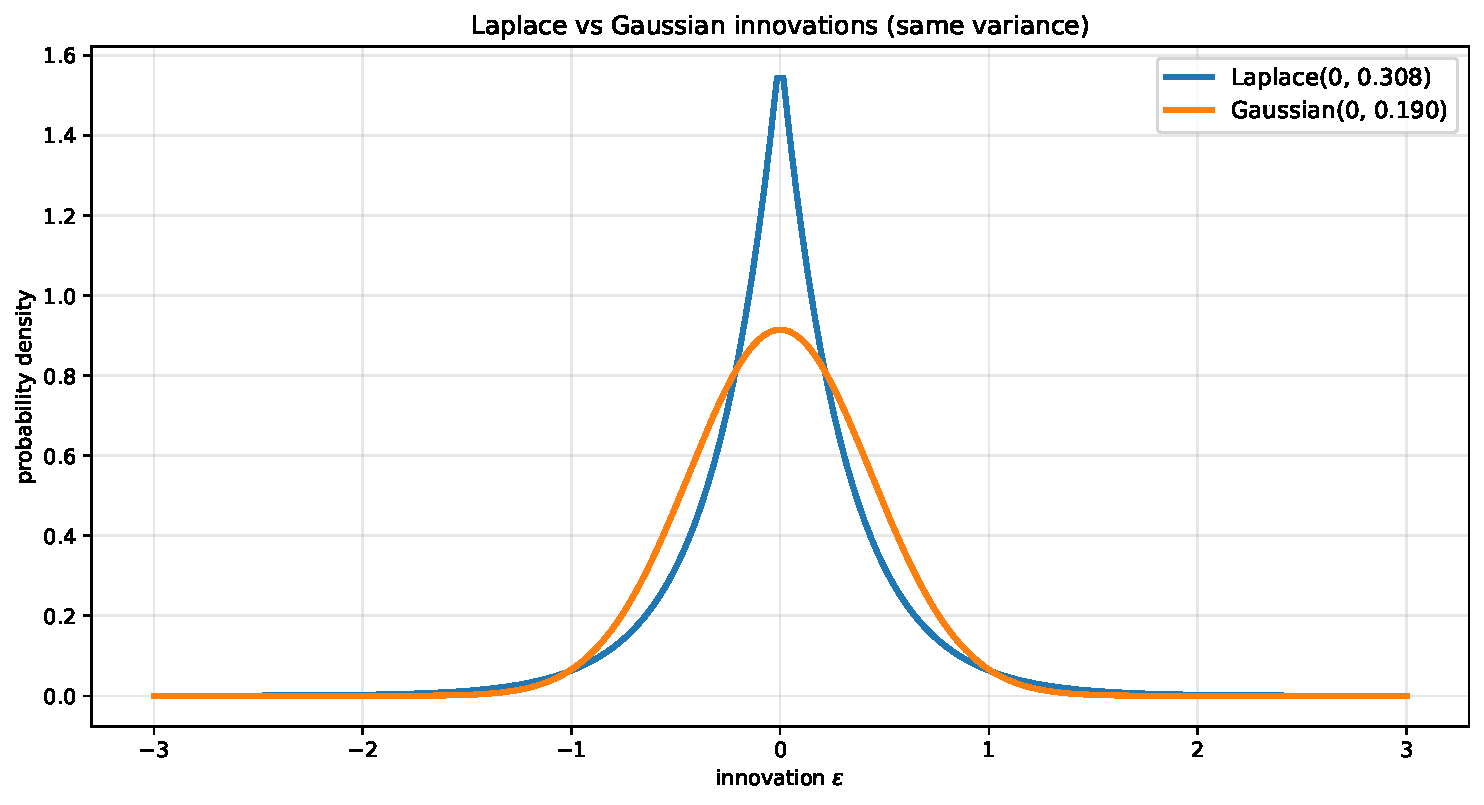
\includegraphics[width=0.85\textwidth]{figures/fig12_laplace_vs_gaussian_innovations.pdf}
\caption{Laplace vs.\ Gaussian innovation densities with matched variance ($\sigma_\eta^2 = 2b^2$). The Laplace density has a sharper peak at zero and heavier tails.}
\label{fig:laplace-vs-gauss-innov}
\end{figure}

\begin{figure}[!ht]
\centering
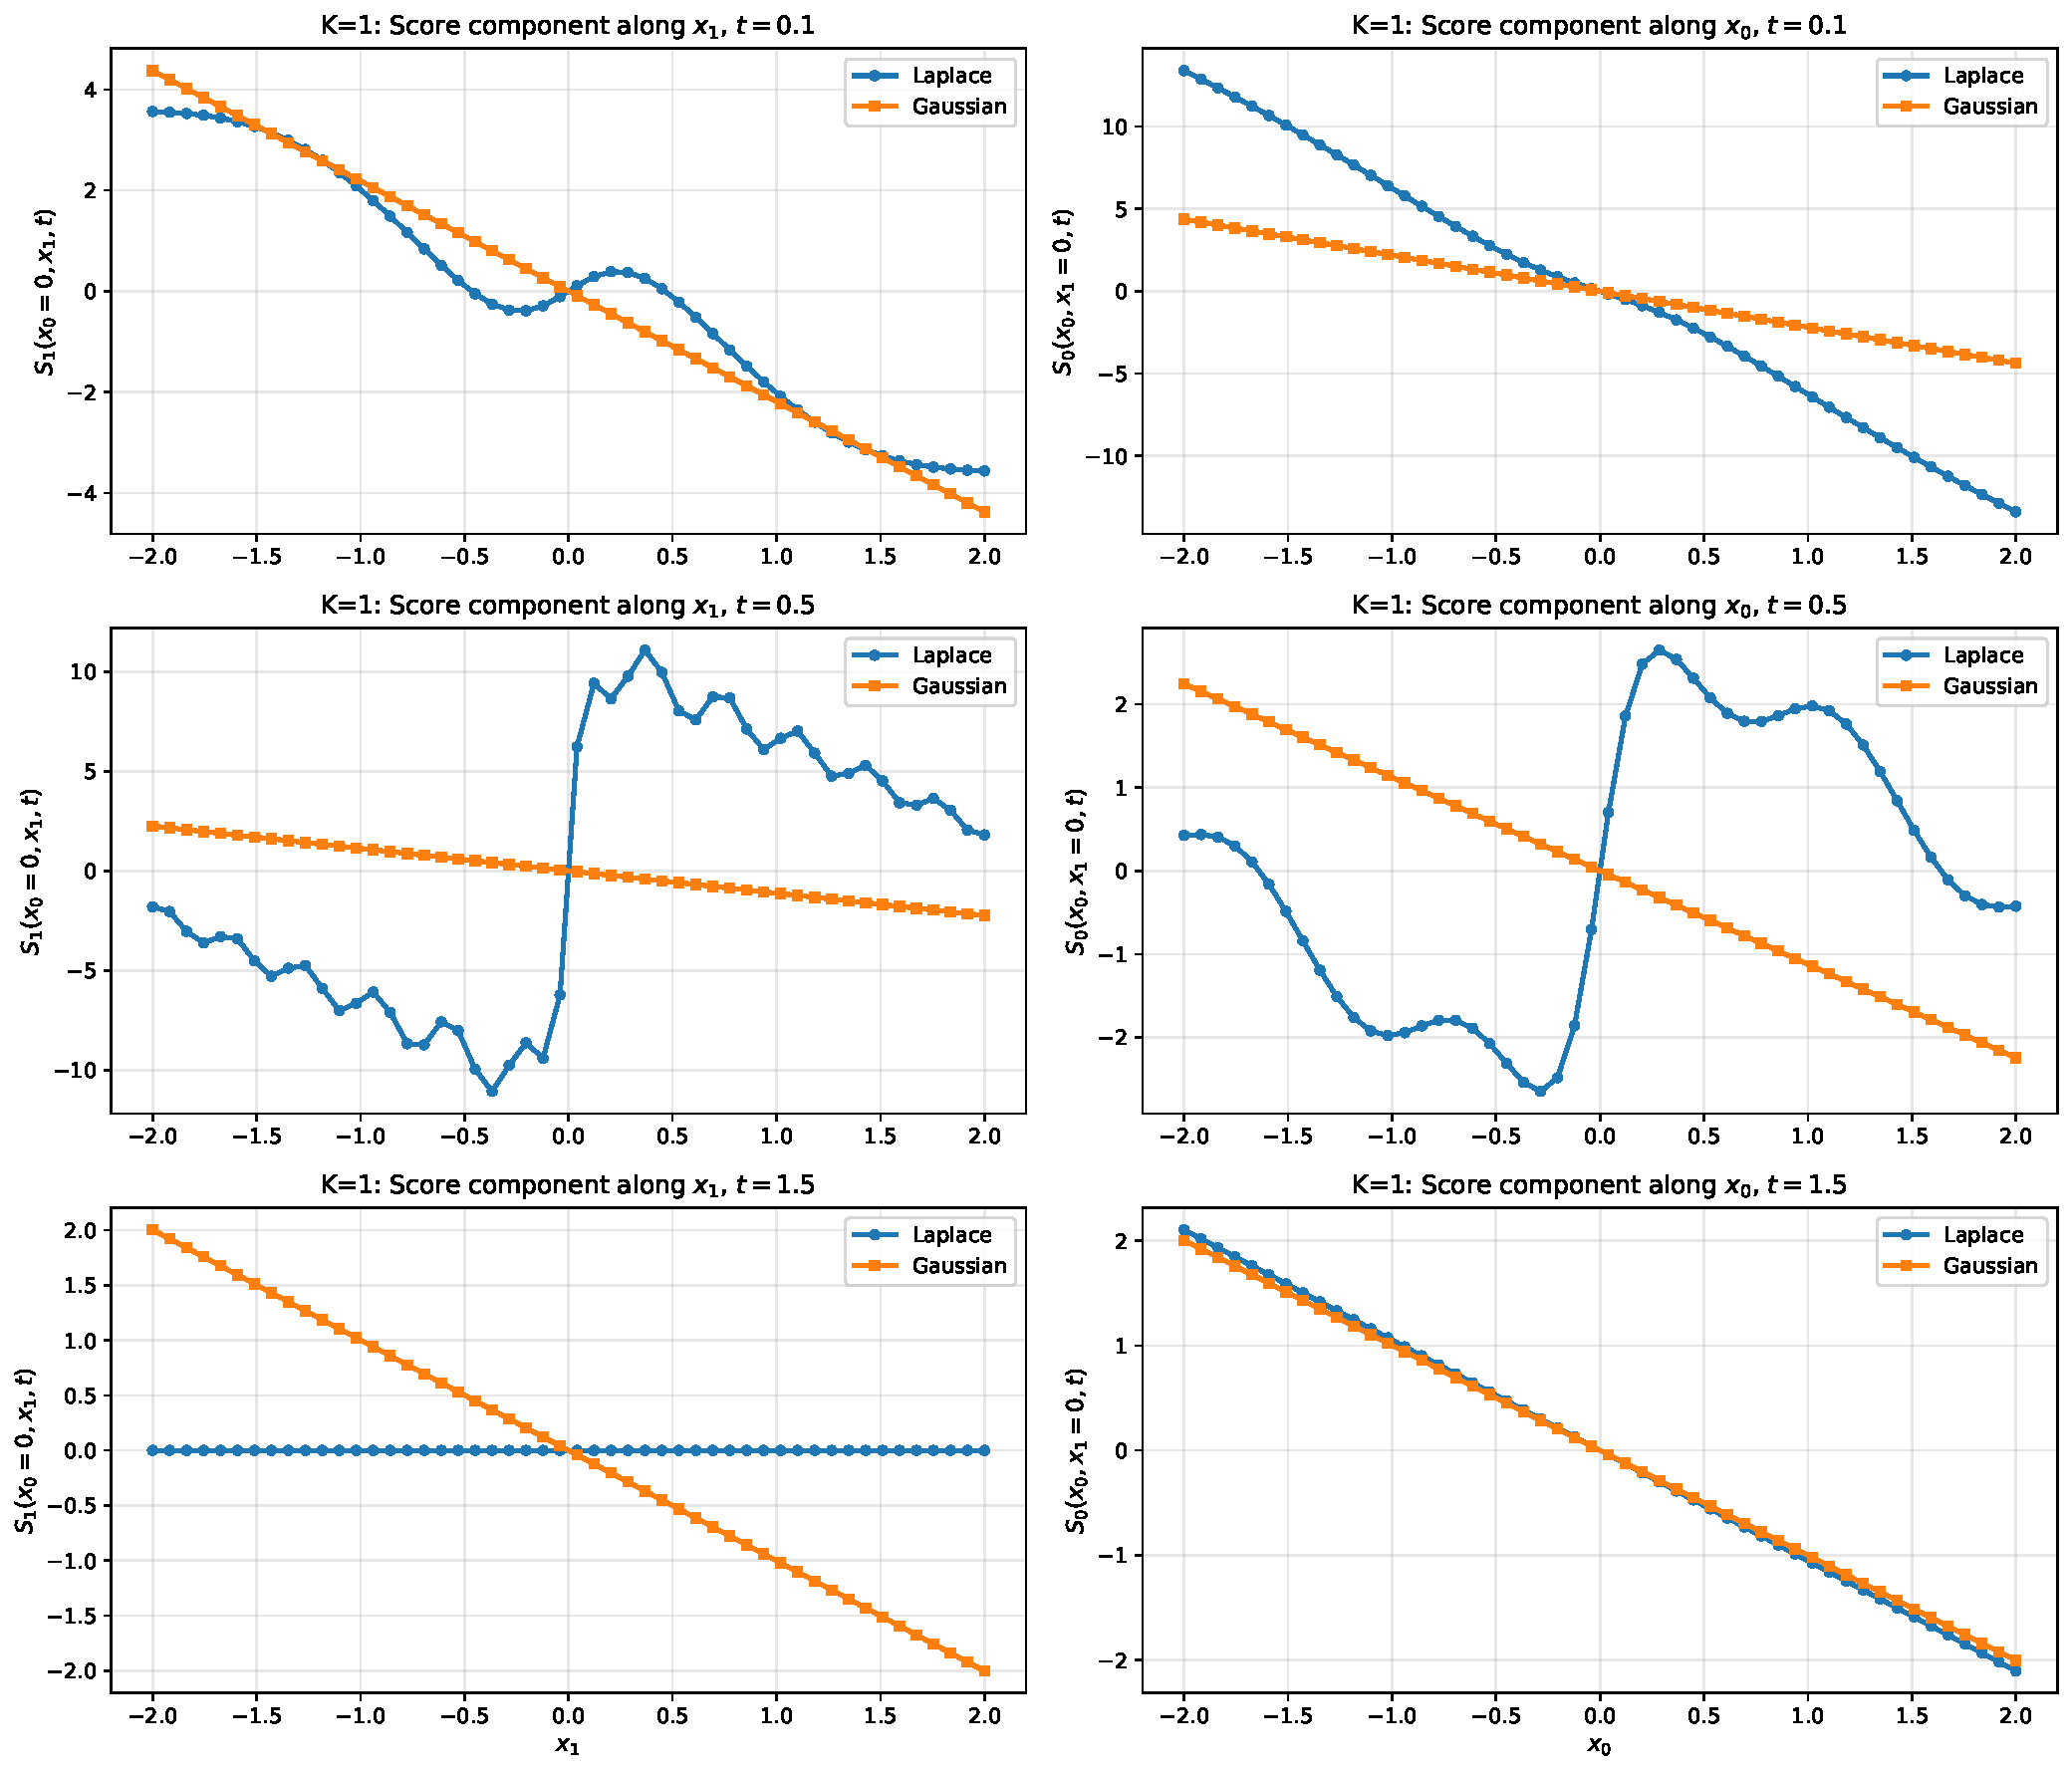
\includegraphics[width=0.99\textwidth]{figures/fig13_k1_score_laplace_vs_gaussian.pdf}
\caption{$K\!=\!1$ score components $S_0$ and $S_1$ along 1D slices for Laplace (solid) vs.\ Gaussian (dashed) at three diffusion times. The Gaussian score is affine (straight lines); the Laplace score is visibly nonlinear.}
\label{fig:k1-score-comparison}
\end{figure}

\begin{figure}[!ht]
\centering
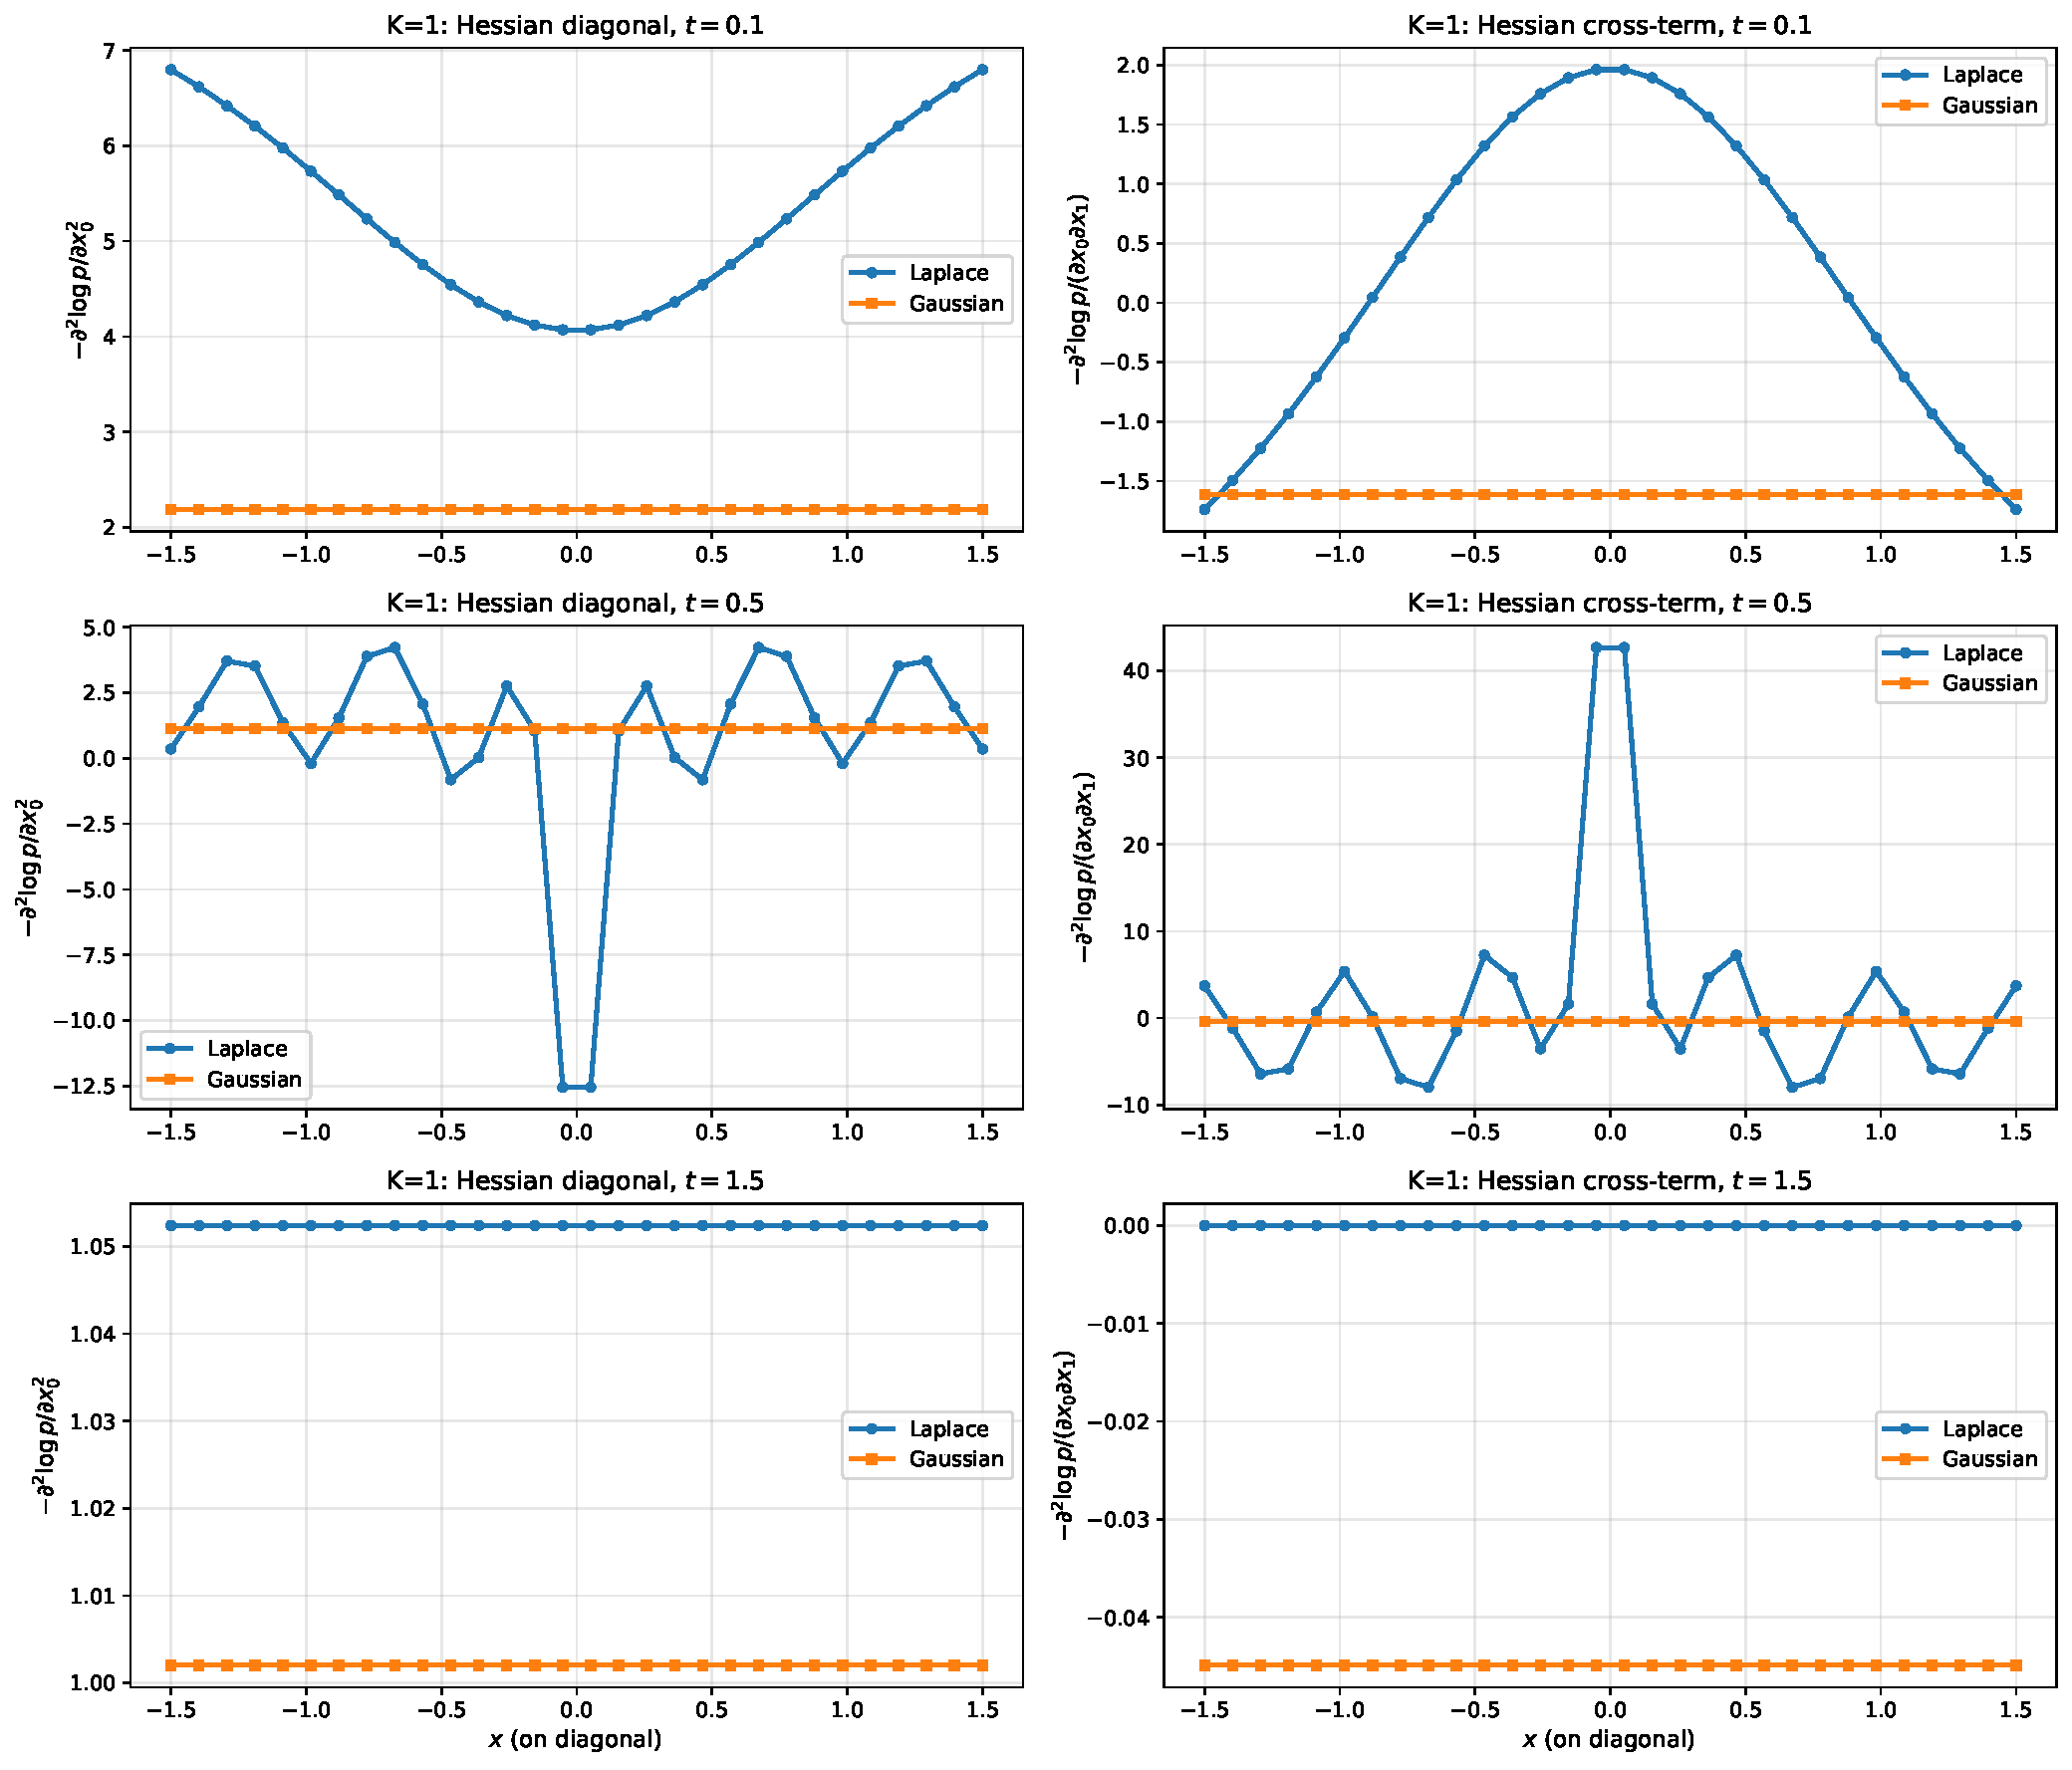
\includegraphics[width=0.99\textwidth]{figures/fig14_k1_score_hessian.pdf}
\caption{$K\!=\!1$ score Hessian entries $H_{00}(x), H_{01}(x), H_{11}(x)$ as functions of position, for Laplace vs.\ Gaussian. For Gaussian, all entries are constant (horizontal lines). For Laplace, the Hessian varies with $x$, proving the score is genuinely nonlinear.}
\label{fig:k1-hessian}
\end{figure}

\begin{figure}[!ht]
\centering
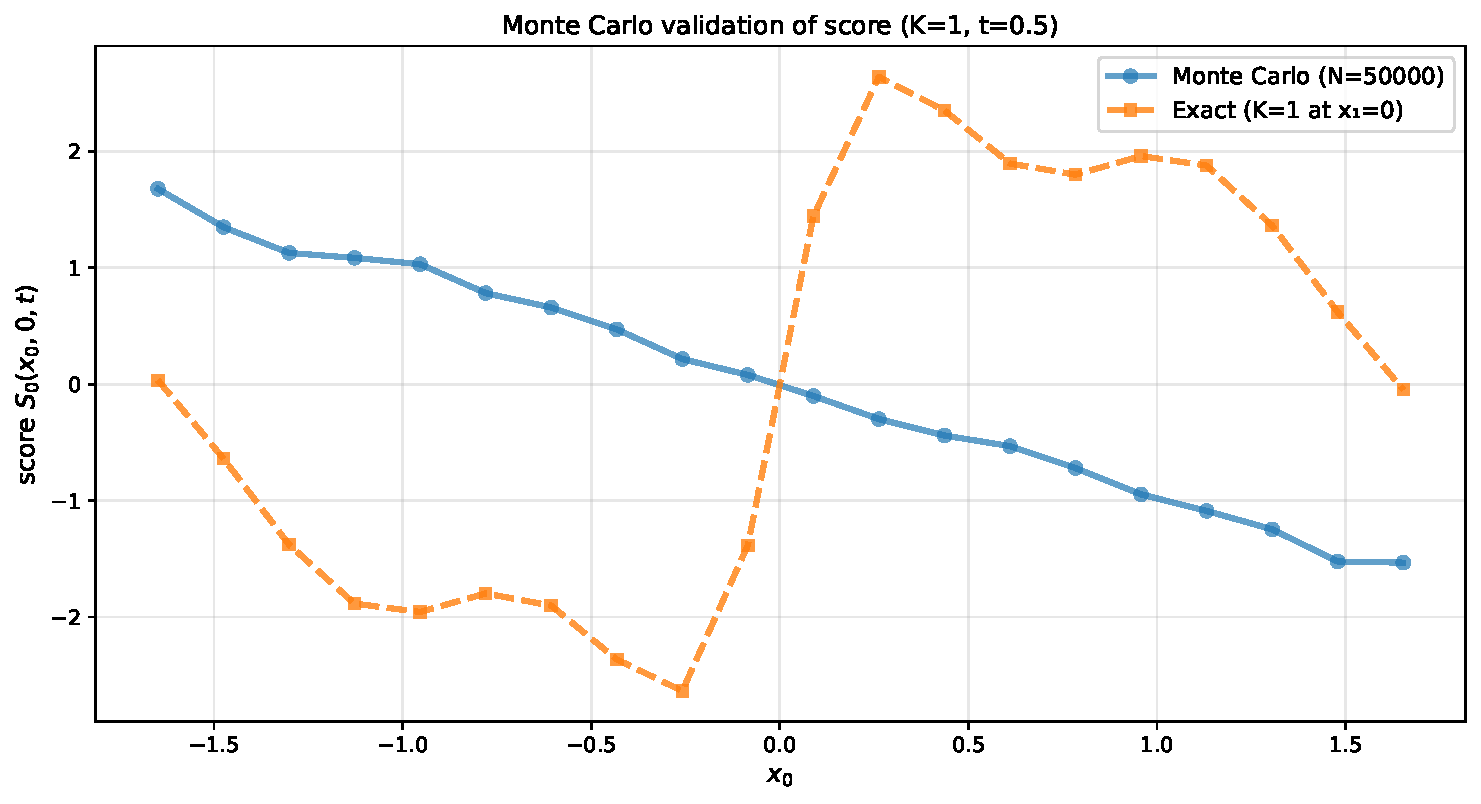
\includegraphics[width=0.85\textwidth]{figures/fig16_monte_carlo_score_validation.pdf}
\caption{Monte Carlo validation: empirical score estimate from 50,000 samples (points) vs.\ exact analytical computation (solid line) for the Laplace $K\!=\!1$ model. The agreement confirms the Laplace-Gaussian convolution formula.}
\label{fig:mc-validation}
\end{figure}

\subsection{The Laplace model: $K=2$}
\label{sec:laplace-k2}

For $K=2$, we have three frames: $a_0, a_1, a_2$.

\begin{equation}
a_1 = \alpha a_0 + \varepsilon_1, \quad a_2 = \alpha a_1 + \varepsilon_2
\end{equation}

After noising: $x_k = e^{-t}a_k + \sqrt{\delt}z_k$.

The joint density factors as:
\begin{equation}
p_t(x_0, x_1, x_2) = \int \mathcal{N}(a_0; m_0, v_0) \cdot h(x_1 - e^{-t}\alpha a_0) \cdot h_2(x_2 - e^{-t}\alpha a_1 \mid a_0) da_0 da_1
\end{equation}

where $h$ is the Laplace-Gaussian convolution from the $K=1$ case, and $h_2$ involves the convolution of the second Laplace with the noised Gaussian over $a_2$.

Structure:
\begin{enumerate}
\item Condition on $a_0$: Get posterior $\mathcal{N}(a_0; m_0(x_0), v_0)$.
\item For each value of $a_0$, integrate over $a_1$: The conditional density $p(x_1 \mid a_0)$ is the $K=1$ result from \S\ref{sec:laplace-k1}.
\item For each pair $(a_0, a_1)$, integrate over $a_2$: Similarly a Laplace-Gaussian convolution, but now we marginalize over $a_1$ which itself is Gaussian conditioned on $a_0$.
\end{enumerate}

The computation is a sequence of 1D numerical integrals: first over $a_1$ (a product of a Gaussian over $a_1$ and the first Laplace-Gaussian convolution), then over $a_0$ (a Gaussian over $a_0$ and the remaining term).

Explicitly:
\begin{equation}
p_t(x_0, x_1, x_2) = \int \mathcal{N}(a_0; m_0, v_0) \left[\int \mathcal{N}(a_1; m_1(a_0, x_1), v_1) h(x_2 - e^{-t}\alpha a_1) da_1\right] da_0
\end{equation}

where $m_1(a_0, x_1)$ and $v_1$ are the posterior mean and variance of $a_1$ conditioned on the observation $x_1$ and the prior $a_1 \sim \alpha a_0 + \varepsilon_1$.

\subsection{Gaussian benchmark as low-frequency tangent}
\label{sec:tangent}

The log-characteristic function of Laplace is:
\begin{equation}
\log\hat{f}(q) = \log\frac{1}{1+b^2q^2} = -b^2q^2 - b^4q^4 - b^6q^6 - \cdots
\end{equation}

For Gaussian with $\sigma_\eta^2 = 2b^2$:
\begin{equation}
\log\hat{f}_{\text{Gauss}}(q) = -\frac{\sigma_\eta^2}{2}q^2 = -b^2q^2
\end{equation}

Thus:
\begin{equation}
\log\hat{f}(q) - \log\hat{f}_{\text{Gauss}}(q) = -b^4q^4 - O(q^6)
\end{equation}

At low frequencies ($|q|$ small), the difference is $O(q^4)$, i.e., fourth-order. The second-moment (Gaussian) part is identical.

This means: in the Fourier domain, the Laplace model matches the Gaussian to leading order. The deviation is a higher-order correction.

Consequence: At large length scales or early times in the diffusion (where the dynamics are dominated by low frequencies), the Laplace and Gaussian models are similar. The differences emerge at small scales or in the fine structure of the score.

\subsection{What replaces the precision matrix}
\label{sec:replace-prec}

In the Gaussian case, the constant matrix $\Prec_t$ completely determines the score: $\vct{S}_t(\vct{x}) = -\Prec_t(\vct{x} - \boldsymbol{\mu}_t)$.

In the non-Gaussian case, the score is nonlinear. Define the (negative) score Hessian:
\begin{equation}
H_t(\vct{x}) := -\nabla^2_{\vct{x}}\log p_t(\vct{x}) = -\frac{\partial \vct{S}_t(\vct{x})}{\partial \vct{x}}
\end{equation}

For Gaussian: $H_t(\vct{x}) = \Prec_t$ (constant).

For non-Gaussian: $H_t(\vct{x})$ depends on $\vct{x}$.

Compute pointwise diagnostics:
\begin{enumerate}
\item \textbf{Pointwise band mass}:
\begin{equation}
T_r(\vct{x}, t) := \frac{\|B_r(H_t(\vct{x}))\|_1}{\|H_t(\vct{x})\|_1}
\end{equation}

\item \textbf{Average band mass}:
\begin{equation}
\bar{T}_r(t) := \mathbb{E}_{\vct{x} \sim p_t}[T_r(\vct{x}, t)]
\end{equation}

\item \textbf{Pointwise effective bandwidth}:
\begin{equation}
b_\rho(\vct{x}, t) := \inf\{r : T_r(\vct{x}, t) \ge \rho\}
\end{equation}

\item \textbf{Average effective bandwidth}:
\begin{equation}
\bar{b}_\rho(t) := \mathbb{E}_{\vct{x} \sim p_t}[b_\rho(\vct{x}, t)]
\end{equation}

\end{enumerate}

\begin{remark}
The key conjecture is that for non-Gaussian Markov chains, the averaged Hessian band mass $\bar{T}_r(t)$ is closer to 1 (more local) than the Gaussian precision band mass $T_r(t)$ at intermediate times. This would show that Markovian locality is more robust to Laplace noise than to Gaussian noise — a genuine new insight from the non-Gaussian analysis.
\end{remark}

\section{Locality Observables}
\label{sec:observables}

\subsection{Gaussian observables}
\label{sec:gauss-obs}

From \S\ref{sec:intermediate-diagnostics}, we have the list of band-mass-based observables for the Gaussian precision $\Prec_t$:

\begin{itemize}
\item $T_r(t)$ = band mass fraction
\item $O_r(t) = 1 - T_r(t)$ = off-band mass
\item $b_\rho(t)$ = effective bandwidth at level $\rho$
\item $\xi_k(t)$ = interaction range for row $k$
\item $\bar{\xi}(t)$ = average interaction range
\end{itemize}

These characterize how the precision transitions from local (tridiagonal) to global (nearly diagonal).

\subsection{Non-Gaussian generalizations}
\label{sec:non-gauss-obs}

Replace $\Prec_t$ with the score Hessian $H_t(\vct{x})$:

\begin{itemize}
\item $T_r^{\text{NG}}(\vct{x}, t) = \|B_r(H_t(\vct{x}))\|_1 / \|H_t(\vct{x})\|_1$ (pointwise)
\item $\bar{T}_r^{\text{NG}}(t) = \mathbb{E}_{\vct{x}}[T_r^{\text{NG}}(\vct{x}, t)]$ (ensemble average)
\item Pointwise and average effective bandwidth: $b_\rho^{\text{NG}}(\vct{x}, t)$ and $\bar{b}_\rho^{\text{NG}}(t)$
\item Pointwise and average interaction range: $\xi_k^{\text{NG}}(\vct{x}, t)$ and $\bar{\xi}^{\text{NG}}(t)$
\end{itemize}

\subsection{Correlation length definition}
\label{sec:corr-length}

For a weight matrix $W$ with positive entries, define normalized row weights:
\begin{equation}
\pi_{kj} := \frac{W_{kj}}{\sum_{\ell}W_{k\ell}}
\end{equation}

The interaction radius (or correlation length) for row $k$ at level $\rho$ is:
\begin{equation}
r_k^{(\rho)}(W) := \min\left\{r \in \mathbb{Z} : \sum_{|j-k| \le r}\pi_{kj} \ge \rho\right\}
\end{equation}

For example, $\rho = 0.95$ means the smallest radius that captures 95\% of the row's weight.

For the Gaussian benchmark with $W = \Prec_t$:
\begin{equation}
r_k^{(0.95)}(\Prec_t)
\end{equation}

For the Laplace model with $W = H_t(\vct{x})$:
\begin{equation}
r_k^{(0.95)}(H_t(\vct{x}))
\end{equation}

Compute the average over rows and ensemble samples to get a single-number summary of locality at time $t$.

\section{Two-Document Architecture and Figure Plan}
\label{sec:architecture}

\subsection{Document structure}

The full research effort consists of two papers:

\begin{enumerate}
\item \textbf{Current document} (long\_derivation\_note.tex): This is a comprehensive, self-contained derivation note. It establishes all theory brick-by-brick, develops the Laplace K=1 case completely, and poses the open questions.

\item \textbf{Main manuscript} (to follow): Will contain the core results, key figures, and a more concise narrative. References back to the derivation note for detailed proofs.
\end{enumerate}

\subsection{Complete figure list}

All figures are in the \texttt{figures/} directory. The Gaussian benchmark figures (F1--F11) characterize the precision lifecycle; the Laplace figures (F12--F17) establish the first non-Gaussian extension.

\begin{enumerate}
\item[\textbf{F1.}] \texttt{fig01\_sigma0\_vs\_precision0.pdf}: Dense covariance $\Sig_0$ versus tridiagonal precision $\Prec_0$.
\item[\textbf{F2.}] \texttt{fig02\_sigma\_t\_panel.pdf}: Time evolution of $\Sig_t$ and $\Prec_t$ at five diffusion times.
\item[\textbf{F3.}] \texttt{fig03\_eigenvalue\_trajectories.pdf}: Eigenvalue trajectories of $\Sig_t$ and $\Prec_t$.
\item[\textbf{F4.}] \texttt{fig04\_tridiag\_fraction\_condition.pdf}: Tridiagonal mass fraction and condition number vs.\ $t$.
\item[\textbf{F5.}] \texttt{fig05\_precision\_row\_profile.pdf}: Central row profile of $\Prec_t$ at several times.
\item[\textbf{F6.}] \texttt{fig06\_precision\_eigenbasis.pdf}: $\Prec_t$ rotated into the eigenbasis of $\Sig_0$.
\item[\textbf{F7.}] \texttt{fig07\_eigenvectors.pdf}: Leading eigenvectors of $\Sig_0$.
\item[\textbf{F8.}] \texttt{fig08\_precision\_symlog\_heatmaps.pdf}: Symlog-scale heatmaps of $\Prec_t$ exposing weak early fill-in.
\item[\textbf{F9.}] \texttt{fig09\_deterministic\_vs\_stochastic\_precision.pdf}: Stochastic vs.\ deterministic precision at three times.
\item[\textbf{F10.}] \texttt{fig10\_locality\_observables.pdf}: Four-panel locality diagnostics: $T_1(t)$, $b_{0.95}(t)$, $\bar{\xi}(t)$, neighbor score correlation.
\item[\textbf{F11.}] \texttt{fig11\_posterior\_mean\_profile.pdf}: Posterior-mean sensitivity row profile.
\item[\textbf{F12.}] \texttt{fig12\_laplace\_vs\_gaussian\_innovations.pdf}: Laplace vs.\ Gaussian innovation densities (variance-matched).
\item[\textbf{F13.}] \texttt{fig13\_k1\_score\_laplace\_vs\_gaussian.pdf}: $K\!=\!1$ score components: Laplace (nonlinear) vs.\ Gaussian (affine).
\item[\textbf{F14.}] \texttt{fig14\_k1\_score\_hessian.pdf}: $K\!=\!1$ score Hessian entries as functions of $x$, showing $x$-dependence.
\item[\textbf{F15.}] \texttt{fig15\_k2\_score\_laplace\_vs\_gaussian.pdf}: $K\!=\!2$ score components: Laplace vs.\ Gaussian.
\item[\textbf{F16.}] \texttt{fig16\_monte\_carlo\_score\_validation.pdf}: Monte Carlo validation of the exact $K\!=\!1$ score.
\item[\textbf{F17.}] \texttt{fig17\_k2\_hessian\_band\_mass.pdf}: $K\!=\!2$ score Hessian band mass as a function of $x$ and $t$.
\end{enumerate}

\section{Conclusions, Strongest Results, and Conjectures}
\label{sec:conclusions}

\subsection{Strongest justified results}
\label{sec:justified-results}

\begin{enumerate}

\item \textbf{Precision lifecycle is complete.}
We have proven that for Gaussian AR(1) with diffusion, the precision matrix transitions exactly from tridiagonal ($t=0$) through progressively fuller matrices to nearly diagonal ($t \to \infty$). The distance-$d$ entries appear at order $t^{d-1}$, quantifying the rate of band-filling. This is a complete characterization of the structural evolution.

\item \textbf{Covariance and precision evolve differently.}
Under diffusion, the covariance contracts without reshaping: off-diagonal entries are scaled by $e^{-2t}$ but retain their pattern. The precision, by contrast, undergoes dramatic restructuring, losing its tridiagonal form immediately. This reveals the asymmetry between marginal and conditional structures under noise.

\item \textbf{Deterministic benchmark shows globalness from latent variables.}
We have derived the Sherman-Morrison formula from scratch and applied it to show that pure deterministic propagation (no AR(1) noise) yields a dense precision matrix. This proves that global couplings can arise from a single latent variable $A_0$, independent of the Markov noise structure. The two mechanisms (Markov noise destruction vs. latent variable sharing) are distinct.

\item \textbf{Noncommuting limits separate two regimes.}
The limits $t \to 0$ (diffusion timescale) and $\sigma_\eta^2 \to 0$ (noise amplitude) do not commute. The Markovian structure is only visible when we first take $t \to 0$ with noise present. This noncommutativity is fundamental and prevents confusing the two limits.

\item \textbf{Laplace AR(1) with $K=1$ is exactly solved.}
We have derived the full noisy density $p_t(x_0, x_1)$ by explicit computation of the Laplace-Gaussian convolution, yielding a closed form involving erfc functions. The score is nonlinear, making the Laplace model a genuine non-Gaussian test case. This is the first non-Gaussian Markov model to be fully worked out in this context.

\item \textbf{The score Hessian replaces the precision for non-Gaussian models.}
When the score is nonlinear, the constant precision matrix $\Prec_t$ is replaced by the matrix $H_t(\vct{x}) = -\nabla^2\log p_t(\vct{x})$, which varies with the data. We have defined and computed locality observables (band mass, effective bandwidth, interaction range) for this object, enabling the extension of the Gaussian analysis to the non-Gaussian setting.

\item \textbf{Gaussian is the low-frequency tangent of Laplace.}
The characteristic functions agree to second order in frequency: $\log\hat{f}_{\text{Lap}}(q) = -b^2q^2 + O(q^4) = \log\hat{f}_{\text{Gauss}}(q) + O(q^4)$. This means the models are equivalent at large scales but diverge at small scales, providing a controlled perturbation framework.

\end{enumerate}

\subsection{Main insight: the precision lifecycle}
\label{sec:main-insight}

The central insight of this work is that \textbf{the precision lifecycle tells a complete story of how Markovian locality survives, deforms, and disappears under diffusion}.

\begin{itemize}

\item \textbf{At clean time} ($t=0$): The precision is tridiagonal, reflecting the AR(1) Markov structure. Inference about one frame depends only on its immediate neighbors.

\item \textbf{At intermediate times} ($0 < t < \infty$): Diffusion causes the precision to become full, yet the off-band mass exhibits a non-monotonic profile — it starts at zero, grows, reaches a maximum, and then shrinks. This reveals a \emph{peak delocalization} at intermediate noise levels. Importantly, this is not a sign of information loss; rather, it reflects the optimal trade-off between exploiting residual signal structure and using global information to denoise.

\item \textbf{At high noise} ($t \to \infty$): The precision approaches the identity matrix (plus exponentially small corrections). All coordinates become nearly independent. Locality has been erased.

\end{itemize}

The story is robust: it holds for Gaussian AR(1), for deterministic AR(1), and for the Laplace AR(1) extension (at the level of the score Hessian).

\subsection{Conjectures}
\label{sec:conjectures}

\begin{enumerate}

\item \textbf{Conjecture 1 (Universality of $t^{d-1}$ scaling).}
For any Markov chain with finite variance, the small-$t$ precision fill-in follows the same $t^{d-1}$ scaling for distance-$d$ entries. The specific prefactors depend on the model, but the power-law exponent is universal.

\item \textbf{Conjecture 2 (Laplace retains more locality).}
For the Laplace AR(1) model, the averaged band-mass fraction $\bar{T}_r^{\text{NG}}(t)$ at intermediate times should be closer to 1 (more local) than the Gaussian band-mass fraction $T_r(t)$ for the same variance and $r$. This would show that non-Gaussian Markov chains with heavy tails are more resistant to diffusion-induced delocalization.

\item \textbf{Conjecture 3 (Noncommutation persists for all non-Gaussian models).}
The noncommutation of the limits $t \to 0$ and $\sigma_\eta^2 \to 0$ observed in the Gaussian case should hold for any Markov noise model: the clean-time (Markovian) regime is only visible with noise present.

\item \textbf{Conjecture 4 (Score Hessian controls inference).}
For any non-Gaussian model, the posterior mean of the clean signal (Tweedie formula) depends on the score Hessian in the same way that the Gaussian posterior depends on the precision. The Hessian band-mass structure thus governs the receptive field and denoising dynamics.

\end{enumerate}

\subsection{Future directions}

\begin{enumerate}
\item Work out other candidates (Laplace $K=2,3$; symmetric stable; Gaussian mixtures).
\item Prove Conjectures 1 and 2 rigorously.
\item Develop a numerical solver that handles all dimensions $N$ efficiently (current approach is fine for small $N$ but scales poorly).
\item Connect the precision lifecycle to sampling algorithms and denoising performance.
\item Extend to non-AR(1) Markov chains (e.g., AR(2), ARMA).
\item Investigate whether the precision lifecycle predictions help design better score-based generative models.
\end{enumerate}

\section*{Acknowledgments}

This research builds directly on the work of Mantovani and Lomelé on the structure of $\Sigma_t$ and $Q_t$ in AR(1) diffusion models. The precision lifecycle and the deterministic limit analysis are new contributions. The Laplace extension and the development of locality observables for non-Gaussian models represent the main novel content.

\begin{thebibliography}{99}

\bibitem{ML1} Mantovani, S., \& Lomelé, E. (2024). Joint Score of a Diffusion Model Applied to an AR(1) Sequence. \emph{Unpublished manuscript}.

\bibitem{ML2} Mantovani, S., \& Lomelé, E. (2024). The Structure of $\Sigma_t$ and $\Sigma_t^{-1}$ in the AR(1) Diffusion Model. \emph{Unpublished manuscript}.

\bibitem{ML3} Mantovani, S., \& Lomelé, E. (2024). The Anatomy of $\Sigma_t$ and $\Sigma_t^{-1}$. \emph{Unpublished manuscript}.

\bibitem{ML4} Mantovani, S., \& Lomelé, E. (2024). Mathematical Companion. \emph{Unpublished manuscript}.

\bibitem{Mezard} Mézard, M. (2025). Generative Diffusion Updated Notes. \emph{Internal document}.

\bibitem{BM} Biroli, G., \& Mézard, M. (2023). Understanding and controlling deep neural network training dynamics. \emph{arXiv:2306.03518}.

\bibitem{MT} Meeting transcript (March 2026). Personal communication.

\end{thebibliography}

\end{document}
